% ---------------------------------------------------------------------------
% Splatt3R-SLAM -- MSc thesis (monograph) build.
%
%   ./build.sh master     -> master.pdf
%
% Independent MSc monograph. RA-L has its own IEEE drivers and prose.
% Both documents reuse measured tabular data and scientific figures only;
% chapter structure, captions, bibliography style and layout belong here.
%
% Fonts: URW Nimbus Roman via `times`, i.e. only distribution-bundled Type 1
% fonts.  Builds identically with pdflatex on Linux (TeX Live) and Windows
% (MiKTeX).  Do NOT switch to XeLaTeX/fontspec.
% ---------------------------------------------------------------------------
\documentclass[12pt,a4paper,oneside]{report}

\usepackage[a4paper,margin=2.5cm]{geometry}
\usepackage{times}
\usepackage[T1]{fontenc}
\usepackage[utf8]{inputenc}
\usepackage{setspace}
\onehalfspacing
\setlength{\emergencystretch}{3em}
\hyphenpenalty=50
\tolerance=1200

\usepackage{graphicx}
\usepackage{amsmath}
\usepackage{amssymb}
\usepackage{booktabs}
\usepackage{multirow}
\usepackage{xcolor}
\usepackage{tikz}
\usetikzlibrary{arrows.meta,calc,backgrounds}
\usepackage{longtable}
\usepackage[numbers,sort&compress]{natbib}
\usepackage[format=plain,labelformat=simple,labelsep=period,font=small]{caption}
\usepackage[font=footnotesize,subrefformat=parens]{subcaption}
\usepackage{microtype}
\usepackage{fancyhdr}
\usepackage{emptypage}

\definecolor{uvared}{rgb}{0.72,0.11,0.11}
\usepackage[pagebackref,breaklinks,colorlinks,citecolor=uvared,linkcolor=uvared,
            urlcolor=uvared]{hyperref}
\usepackage[capitalize]{cleveref}
\hypersetup{pdftitle={Splatt3R-SLAM: From Image Pairs to Persistent Maps},
            pdfauthor={Zelong Li}}

% Table macros, shared with the paper build.
\newcommand{\best}[1]{\textbf{#1}}
\newcommand{\dB}{\,dB}
\newcommand{\up}{$\uparrow$}
\newcommand{\dn}{$\downarrow$}

% Front-matter (\chapter*) headings: report's default drops 50pt of white
% space above the title, which on an A4 page with 1.5 spacing pushes short
% front-matter chapters onto a second page. 10pt is enough to read as a break.
% Numbered chapter heads: report drops 50pt above "Chapter N" and 20pt below
% the title. On A4 at 1.5 spacing that is close to four lines of text per
% chapter, which is what pushes short chapter tails onto a page of their own.
\makeatletter
\renewcommand{\@makechapterhead}[1]{%
  \vspace*{16\p@}%
  {\parindent \z@ \raggedright \normalfont
   \ifnum \c@secnumdepth >\m@ne
     \Large\bfseries \@chapapp\space \thechapter
     \par\nobreak
     \vskip 8\p@
   \fi
   \interlinepenalty\@M
   \Huge \bfseries #1\par\nobreak
   \vskip 24\p@}}
\renewcommand{\@makeschapterhead}[1]{%
  \vspace*{10\p@}%
  {\parindent \z@ \raggedright \normalfont
   \interlinepenalty\@M
   \Huge\bfseries #1\par\nobreak
   \vskip 24\p@}}
\makeatother

% Running heads.
\pagestyle{fancy}
\fancyhf{}
\renewcommand{\headrulewidth}{0.4pt}
\fancyhead[L]{\small\nouppercase{\leftmark}}
\fancyhead[R]{\small\thepage}
\setlength{\headheight}{15pt}
\fancypagestyle{plain}{\fancyhf{}\renewcommand{\headrulewidth}{0pt}%
  \fancyfoot[C]{\small\thepage}}

% Slightly looser float placement than the two-column paper needs.
\renewcommand{\topfraction}{0.85}
\renewcommand{\textfraction}{0.1}
\renewcommand{\floatpagefraction}{0.75}

\begin{document}

\pagenumbering{roman}
\hypersetup{pageanchor=false}
\begin{titlepage}
\thispagestyle{empty}
\centering
\singlespacing

\vspace*{0.4cm}

{\Large\scshape University of Amsterdam}\\[0.25cm]
{\large Faculty of Science}\\[0.12cm]
{\large MSc Computer Science \emph{(joint degree)}}

\vspace{1.4cm}

{\large Master's Thesis}

\vspace{0.9cm}

\rule{\linewidth}{0.5pt}

\vspace{0.5cm}

{\LARGE\bfseries Splatt3R-SLAM:\\[0.2cm]
From Image Pairs to Persistent Maps\par}

\vspace{0.5cm}

\rule{\linewidth}{0.5pt}

\vspace{1.4cm}

{\large\bfseries Zelong Li}\\[0.2cm]
{\normalsize \texttt{loong.li2@student.uva.nl}}\\[0.1cm]
{\normalsize \texttt{+31\,6\,3023\,2998}}\\[0.1cm]
{\normalsize Student number 15326322}

\vspace{1.4cm}

\begin{tabular}{@{}ll@{}}
\emph{Supervisor:}       & Prof.\ Martin Oswald\\[0.15cm]
\emph{Daily supervisor:} & Dr.\ Qi Zhang\\[0.15cm]
\emph{Second reader:}    & \emph{[to be assigned --- fill in]}\\
\end{tabular}

\vfill

{\normalsize Submitted in partial fulfilment of the requirements\\
for the degree of Master of Science}

\vspace{0.8cm}

{\normalsize \today}

\vspace{0.4cm}
\end{titlepage}

\hypersetup{pageanchor=true}

\chapter*{Abstract}
\addcontentsline{toc}{chapter}{Abstract}
\markboth{Abstract}{Abstract}
\begin{singlespace}

An image pair can now produce a dense 3D Gaussian reconstruction in one
network pass. A video instead creates overlapping predictions that must follow
loop-closure corrections. This thesis presents Splatt3R-SLAM, a monocular
system that turns local predictions into a persistent map. It gives each
local Gaussian map and its observation cameras the same keyframe anchor, so
pose corrections move both together. A separate process refines appearance
while MASt3R-SLAM estimates motion.

Head-only adaptation changes prediction, opacity attenuation changes
insertion, and photometric refinement uses sequence observations. Refinement
improves PSNR by $1.00$--$8.69$\,dB across four controls. Attenuation
improves LPIPS in ten of twelve tests, although confidence weighting offers
little advantage over uniform attenuation.

Under common non-keyframe reconstruction evaluation, the released head with
$300$\,s refinement reaches $23.02$\,dB mean PSNR on eight Replica scenes,
compared with $19.48$\,dB for Photo-SLAM. On TUM desk, its $13.95$\,dB is
close to MonoGS, which has lower LPIPS. Dense prediction provides a useful
initialisation but creates millions of primitives. Compact online mapping
remains the main open problem.
\end{singlespace}

\chapter*{Acknowledgements}
\addcontentsline{toc}{chapter}{Acknowledgements}
\markboth{Acknowledgements}{Acknowledgements}

\emph{[This page is a placeholder to be personalised before submission.]}

I would like to thank my supervisors and second reader for their guidance.
I also thank the authors and maintainers of MASt3R-SLAM, Splatt3R, MonoGS,
Photo-SLAM, and VGGT-SLAM for making their research code available.


\tableofcontents
\listoffigures
\listoftables
\chapter*{Notation and Abbreviations}
\addcontentsline{toc}{chapter}{Notation and Abbreviations}
\markboth{Notation and Abbreviations}{Notation and Abbreviations}

\begin{center}
\begin{tabular}{@{}ll@{}}
\toprule
Symbol & Meaning \\
\midrule
$I_t$                  & RGB image of frame $t$ \\
$\mathbf{X}_t$         & pointmap predicted for frame $t$, in some frame's coordinates \\
$c_n,\hat{c}_n$        & raw confidence and its within-keyframe normalised rank \\
$\alpha_n$             & predicted opacity of Gaussian $n$ \\
$\alpha'_n$            & opacity after injection-time thinning \\
$\lambda$              & thinning strength, \texttt{--refiner-conf-fade} \\
$\lambda_D$            & D-SSIM weight in the refinement objective \\
$\mathbf{T}_{wc}$      & camera-to-world pose, $\mathrm{SE}(3)$ or $\mathrm{Sim}(3)$ \\
$s_k$                  & scale of keyframe cluster $k$ \\
$\mathcal{L}_{\text{ref}}$ & online refinement objective \\
$\hat{I}$              & rendered image \\
\midrule
Abbrev. & Expansion \\
\midrule
3DGS   & 3D Gaussian Splatting \\
ATE    & Absolute Trajectory Error \\
D-SSIM & structural dissimilarity, $1-\mathrm{SSIM}$ \\
GS     & Gaussian Splatting \\
LPIPS  & Learned Perceptual Image Patch Similarity \\
LoRA   & Low-Rank Adaptation \\
PSNR   & Peak Signal-to-Noise Ratio \\
RMSE   & Root-Mean-Square Error \\
SLAM   & Simultaneous Localisation and Mapping \\
SSIM   & Structural Similarity Index Measure \\
\bottomrule
\end{tabular}
\end{center}


\cleardoublepage
\pagenumbering{arabic}
\setcounter{page}{1}

\chapter{Introduction}
\label{ch:intro}

\begin{figure}[t]
  \centering
  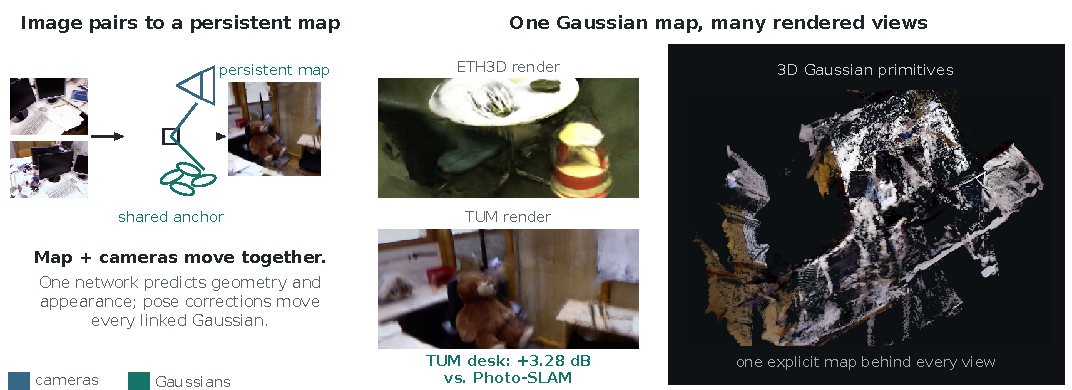
\includegraphics[width=\linewidth]{ral/fig/teaser.pdf}
  \caption[From local predictions to a persistent map]{Splatt3R-SLAM
  predicts local Gaussian maps, carries them with keyframe anchors, and
  refines their appearance. The image is a middle-ranked Replica office0
  comparison. The chart reports all eight Replica scenes with common
  non-keyframe cameras and full exported SH.}
  \label{fig:teaser}
\end{figure}

A robot map must remain useful after the camera has left a room. It must
support localisation, preserve scene structure, and show what the scene
looks like from another viewpoint. Classical visual SLAM provides camera
motion and geometry. 3D Gaussian splatting~\cite{kerbl20233dgs} adds a
renderable appearance model.

Most Gaussian SLAM systems build this model through per-scene optimisation.
MonoGS~\cite{matsuki2024monogs}, Photo-SLAM~\cite{huang2024photoslam}, and
related systems create and update primitives as images arrive.
Feed-forward reconstruction offers another starting point.
DUSt3R~\cite{wang2024dust3r} and MASt3R~\cite{leroy2024mast3r} predict dense
geometry from image pairs. Splatt3R~\cite{smart2024splatt3r} extends the same
features with Gaussian position, shape, colour, and opacity.

This pairwise capability changes the cost of map creation, but it leaves a
sequence-level problem. Every image pair defines a local coordinate frame.
Repeated observations create overlapping copies of the same surface.
Later loop closures move earlier camera poses. Simply concatenating the
predictions therefore produces a large map whose placement and appearance
can become inconsistent.

\section{The central idea}

Splatt3R-SLAM gives every local map a keyframe anchor. Its Gaussians remain
in that anchor's coordinates and move when the pose graph updates the
keyframe. The images used to refine the map are stored relative to the same
anchors. A pose correction then moves the local map and its observation
cameras together.

This shared-anchor relation is the thread through the thesis. It connects
pairwise prediction to a persistent map, allows appearance refinement to
run after tracking, and gives each experiment a clear role. The system
follows three stages:
\begin{enumerate}\itemsep3pt
\item \textbf{Predict} a local Gaussian map from an image pair.
\item \textbf{Anchor} the map and its supervision to the pose graph.
\item \textbf{Refine} Gaussian appearance against tracked RGB observations.
\end{enumerate}
The geometric tracker remains MASt3R-SLAM~\cite{murai2025mast3rslam}.
The mapping process reads its poses but does not optimise them.

\section{Research questions}
\label{sec:intro:rq}

The experiments address four questions:
\begin{description}\itemsep4pt
\item[RQ1] How can pairwise Gaussian prediction be adapted without changing
the shared geometric features used for tracking?
\item[RQ2] Can opacity attenuation at insertion reduce the effect of
overlapping predictions in an assembled map?
\item[RQ3] How much appearance improvement comes from sequence-level
refinement, and can it be delivered without disrupting tracking?
\item[RQ4] How does the complete system compare with locally executed SLAM
baselines in rendering quality, trajectory accuracy, map size, and compute?
\end{description}

\section{From design to evidence}

Each chapter tests one part of the pipeline. Head-only adaptation changes
the first stage while the encoder and decoder stay frozen. Opacity thinning
changes the second stage by lowering the initial contribution of selected
primitives. The refiner changes the third stage through an RGB rendering
loss. Paired studies isolate these interventions before the complete system
is compared with other methods.

The main external result uses the released Splatt3R head, no thinning,
fixed Gaussian centres, and $300$\,s post-sequence refinement. Under common
non-keyframe reconstruction evaluation, its mean PSNR on eight Replica
scenes is $23.02$\,dB, compared with $19.48$\,dB for Photo-SLAM.
On TUM desk, its $13.95$\,dB is close to MonoGS's $13.91$\,dB, while
MonoGS has lower LPIPS. The same evaluation also exposes the cost of dense
prediction: the TUM map contains $2.397$ million primitives.

\section{Contributions}
\label{sec:intro:contrib}

\begin{enumerate}\itemsep4pt
\item A pose-anchored mapping design in which local Gaussians and their
supervision cameras follow the same keyframe corrections
(\cref{ch:system,ch:refiner}).
\item A decoupled refinement process that improves appearance without
updating the tracking model or camera poses, with causal, latency, and
two-GPU controls (\cref{ch:refiner,ch:results}).
\item Paired studies of head-only adaptation and insertion-time opacity
attenuation, including controls for confidence weighting and refinement
(\cref{ch:adapt,ch:thin}).
\item Common-camera reconstruction comparisons with all-eight-scene Replica
coverage, four-method qualitative views, trajectory controls, and explicit
map-size and resource measurements (\cref{ch:protocol,ch:results}).
\end{enumerate}

\section{Thesis structure}

\Cref{ch:bg,ch:related} introduce Gaussian rendering, pairwise prediction,
and related SLAM systems. \Cref{ch:system} presents the shared-anchor design.
\Cref{ch:adapt,ch:thin,ch:refiner} explain the three intervention stages.
\Cref{ch:protocol,ch:results} define and report the evaluation.
\Cref{ch:negative} records tested routes that did not improve the complete
system. \Cref{ch:discussion,ch:conclusion} discuss the remaining problems
and future work. The appendices contain configurations, reproduction steps,
baseline build records, and extended tables.

\chapter{Background}
\label{ch:bg}

This chapter introduces the representation, renderer, prediction models, and
tracking system used by Splatt3R-SLAM. It also defines the metrics used in
later experiments.

\section{3D Gaussian splatting}
\label{sec:bg:3dgs}

\subsection{The representation}

3D Gaussian splatting~\cite{kerbl20233dgs} represents a scene as an unordered
set of anisotropic Gaussians. Primitive $n$ carries a centre
$\mu_n\in\mathbb{R}^3$, a covariance $\Sigma_n\in\mathbb{R}^{3\times3}$, an
opacity $\alpha_n\in(0,1)$ and a view-dependent colour encoded as
spherical-harmonic coefficients. Its unnormalised spatial influence at a
world point $x$ is
\begin{equation}
G_n(x) \;=\; \exp\!\Bigl(-\tfrac{1}{2}(x-\mu_n)^{\!\top}\Sigma_n^{-1}(x-\mu_n)\Bigr).
\label{eq:gaussian}
\end{equation}
A covariance must remain positive semi-definite under gradient descent.
It is therefore factored into a rotation
unit quaternion $q_n$ and positive per-axis scale $s_n$:
\begin{equation}
\Sigma_n \;=\; R(q_n)\,\operatorname{diag}(s_n^2)\,R(q_n)^\top .
\label{eq:cov}
\end{equation}
The scale is parameterised as $s_n=\exp(\hat{s}_n)$ elementwise, which keeps
it positive without a constraint. Large changes in $\hat{s}_n$ can produce the
scale excursions measured in \cref{sec:neg:lora}.

\subsection{Projection and rasterisation}

Rendering projects each Gaussian to the image plane. Let $R_{\mathcal CW}$ be
the rotation from world coordinates to the rendering camera and let $J_n$ be
the $2\times3$ Jacobian of perspective projection at the transformed centre.
The EWA construction of \citet{zwicker2001ewa} gives
\begin{equation}
\Sigma_n^{2D}
  =J_n R_{\mathcal CW}\Sigma_n^W R_{\mathcal CW}^{\top}J_n^{\top}.
\label{eq:proj}
\end{equation}
The rasteriser sorts primitives by depth per screen tile and composites them
front-to-back. Let $\mathbf c_\ell(u)$ be the SH-evaluated RGB colour and
$b_\ell(u)\in[0,1]$ the opacity multiplied by the 2D Gaussian footprint of the
$\ell$-th primitive along pixel ray $u$. The rendered colour is
\begin{equation}
\hat I(u)=\sum_{\ell=1}^{K}\mathbf c_\ell(u)b_\ell(u)
          \prod_{r<\ell}\bigl(1-b_r(u)\bigr),
\label{eq:alphacomp}
\end{equation}
and the residual transmittance after all $K$ primitives is
\begin{equation}
\mathcal T_{K}(u)=\prod_{\ell=1}^{K}\bigl(1-b_\ell(u)\bigr).
\label{eq:transmittance}
\end{equation}

\subsection{Background and visibility}
\label{sec:bg:black}

\Cref{eq:transmittance} is where the background enters. A renderer composites
$\hat I(u)\leftarrow\hat I(u)+\mathcal T_K(u)\mathbf c_{\mathrm{bg}}$, so with
$\mathbf c_{\mathrm{bg}}=0$ the residual
transmittance contributes \emph{zero radiance}: whatever a ray fails to hit is
black. For one isolated primitive with non-negative colour, increasing
opacity increases its contribution against that background. A stack is more
general: changing one opacity also changes the visibility of every primitive
behind it. A darker foreground primitive can hide a brighter background
primitive, so increasing its opacity can lower pixel luminance.
Opacity affects appearance as well as coverage, but the sign cannot be
inferred from the background alone. This distinction limits the
interpretation of the experiments in \cref{ch:thin}.

\subsection{Per-scene optimisation, and what a feed-forward model skips}

The reference 3DGS pipeline initialises primitives from a structure-from-motion
point cloud and optimises them against posed training images under
\begin{equation}
\mathcal{L}_{\text{3DGS}} = (1-\lambda_D)\,\lVert\hat{I}-I\rVert_1
      + \lambda_D\bigl(1-\mathrm{SSIM}(\hat{I},I)\bigr),
\label{eq:3dgsloss}
\end{equation}
interleaved with \emph{adaptive density control}: primitives whose view-space
positional gradient exceeds a threshold are cloned (if small) or split (if
large), primitives whose opacity falls below a threshold are pruned, and
opacity is periodically reset so that the optimiser must re-justify every
primitive it keeps. Spherical-harmonic degree is raised on a schedule, so that
low-frequency appearance is fitted before view-dependent effects.

A feed-forward model emits all primitives in one pass. It has no per-scene
densification, pruning schedule, or opacity reset. When predictions from many
keyframes are accumulated, the map therefore retains every inserted
primitive. \Cref{sec:lim:compact} measures the resulting size.
Our online refiner (\cref{ch:refiner}) restores the image objective in
\cref{eq:3dgsloss}, but not adaptive density control.

\section{Feed-forward pointmaps and Gaussians}
\label{sec:bg:feedforward}

\subsection{DUSt3R and MASt3R}

DUSt3R~\cite{wang2024dust3r} maps an uncalibrated image pair
$I_i,I_j\in\mathbb{R}^{H\times W\times3}$ to pointmaps
$X_{\mathcal C_i}^{(i)},X_{\mathcal C_i}^{(j)}
\in\mathbb{R}^{H\times W\times3}$ with confidences
$C_{\mathcal C_i}^{(i)},C_{\mathcal C_i}^{(j)}$. Here
$X_{\mathcal C_a}^{(b)}$ denotes image $b$'s pointmap expressed in camera
frame $\mathcal C_a$. Both images pass through a shared ViT encoder; two
decoders then attend to each other's tokens, so each view's prediction is
conditioned on the other, and DPT heads regress the pointmaps. The output lives
in the \emph{first} camera's frame, so a single forward pass already encodes
the relative pose implicitly rather than as an explicit estimate.

MASt3R~\cite{leroy2024mast3r} adds a matching head producing dense local
features $D^{(i)},D^{(j)}\in\mathbb{R}^{H\times W\times d}$, trained so that
corresponding pixels are mutual nearest neighbours in feature space. We write
$F_M(I_i,I_j)$ for one forward pass.

Two properties of this family govern everything downstream. The prediction is
\emph{scale-ambiguous up to a per-forward gauge} --- each independent pass
chooses its own scale, and nothing couples the choices --- and it is
\emph{pairwise}, so no single forward pass ever observes more than two views.
\Cref{sec:neg:frontend} measures scale disagreement and finds that joint
multi-view context reduces it in the tested models.

\subsection{Many-view feed-forward models}

VGGT~\cite{wang2025vggt} generalises the formulation: all views enter one
transformer with alternating frame-wise and global attention, and cameras,
depth maps and pointmaps are read out jointly. The consequence that matters
here is that a many-view model solves for a \emph{shared} scale across its
input window instead of drawing one per pair. \Cref{sec:neg:frontend}
quantifies the difference at $6.4\times$ --- and also shows that the same
weights run pairwise are worse than the two-view MASt3R line, so the advantage
belongs to the context, not to the architecture.

\subsection{Splatt3R}

Splatt3R~\cite{smart2024splatt3r} adds a third head, in parallel to the
pointmap and matching heads and using the same DPT decoder, which emits for
pixel $n$ a rotation quaternion $q_n\in\mathbb{R}^4$, a scale
$s_n\in\mathbb{R}_{>0}^3$, spherical-harmonic coefficients
$S_n\in\mathbb{R}^{3\times D_{\mathrm{SH}}}$, an opacity logit
$\widetilde\alpha_n\in\mathbb{R}$, and a mean offset
$\Delta_n\in\mathbb{R}^3$. The Gaussian centre and opacity are
\begin{equation}
\mu_n=x_n+\Delta_n,\quad x_n\in X_{\mathcal C_i}^{(i)},\qquad
\alpha_n=\operatorname{sigmoid}(\widetilde\alpha_n).
\label{eq:mu}
\end{equation}
$D_{\mathrm{SH}}$ is the number of SH basis coefficients per colour channel.
Quaternions are normalised and raw scale channels are exponentiated.
Offsets use a norm-dependent exponential rescaling of a signed vector, so their coordinates
are not restricted to positive values. In upstream training, \emph{only the Gaussian
head is trained}: the encoder and decoder remain those of the pre-trained
MASt3R model, and all Gaussian parameters are predicted in the first image's
camera frame, avoiding any ground-truth transformation at inference.

Covariance follows \cref{eq:cov} and rendering follows
\cref{eq:alphacomp}; the Gaussians a single forward pass emits are therefore
immediately renderable by a standard 3DGS rasteriser, with no optimisation
step in between.

Splatt3R is supervised only by novel-view renderings, under a mask $M$ of
pixels visible in at least one context view:
\begin{equation}
\mathcal{L}_{\mathrm{head}}
  =\mathcal{L}_{\mathrm{MSE},M}(\hat I,I)
  +0.25\,\mathcal{L}_{\mathrm{LPIPS(VGG)},M}(\hat I,I),
\label{eq:splatt3rloss}
\end{equation}
where the subscript $M$ denotes spatial averaging over valid pixels.
Two properties of \cref{eq:splatt3rloss} drive our method.
It is \emph{purely photometric} ---
depth enters only through the mask $M$ and through pair selection, never
through a gradient on geometry --- and it is \emph{pairwise}: the loss never
observes more than two context views, hence never observes a fused map.

In the released implementation the DC colour is anchored to the source image:
the head predicts a residual which is added to the spherical-harmonic encoding
of the input RGB value,
\begin{equation}
S_{\mathrm{DC}}(u)=S_{\mathrm{res}}(u)+\operatorname{RGB2SH}(I_i(u)).
\label{eq:colorresidual}
\end{equation}
Colour is clamped during conversion; it is not sigmoid-bounded. The residual
provides an appearance adjustment independently of opacity, so opacity is
not the only channel capable of compensating for input photometry.
Consequently, revisits can inherit exposure, white-balance, shadow, and
view-dependent differences from their source frames. Exposure normalisation
removes only the global component of this source-frame photometric gauge; it
does not enforce equality of $S_{\mathrm{DC}}$ for the same world surface.


\section{SLAM with a pointmap prior}
\label{sec:bg:slam}

We use $T_{AB}$ for a transform that maps coordinates from frame $B$ to
frame $A$. We use the front- and back-end of
MASt3R-SLAM~\cite{murai2025mast3rslam}. This section summarises the tracking
path whose trajectory accuracy is measured in \cref{ch:results}.

\subsection{Poses on the Sim(3) manifold}

Because network predictions are scale-ambiguous, poses are $\mathrm{Sim}(3)$
rather than $\mathrm{SE}(3)$, so that a per-keyframe scale is available to
absorb the ambiguity:
\begin{equation}
T=\begin{bmatrix} aR & t\\ 0 & 1\end{bmatrix},\qquad
T \leftarrow \tau \oplus T \triangleq \mathrm{Exp}(\tau)\circ T ,
\label{eq:sim3}
\end{equation}
with $a>0$ and $\tau\in\mathfrak{sim}(3)$. The scale degree of freedom
absorbs per-forward gauge error. This is why
\cref{sec:neg:frontend} finds that correcting the map's scales alone makes the
rendering worse.

\subsection{Matching and the ray error}

Under a generic central-camera assumption a pointmap induces its own camera
model through the ray map $\psi(X)=X/\lVert X\rVert$. Two rays differ by
\begin{equation}
\lVert\psi_1-\psi_2\rVert^2 = 2(1-\cos\theta), \qquad \cos\theta=\psi_1^{\!\top}\psi_2,
\label{eq:rayangle}
\end{equation}
which is \emph{bounded}, whereas a 3D point error is not. Since pointmap
predictions exhibit depth errors far more often than directional errors,
tracking minimises a ray error rather than a point error. For matches
$\mathcal M_{f,k}$ between the current frame $f$ and keyframe $k$,
\begin{equation}
E_r=\!\!\sum_{m,n\in\mathcal M_{f,k}}\!\!
\Bigl\lVert
\frac{\psi(\widetilde X_{\mathcal C_k,n}^{(k)})
 -\psi(T_{\mathcal C_k\mathcal C_f}X_{\mathcal C_f,m}^{(f)})}
{w(\omega_{m,n},\sigma_r^2)}
\Bigr\rVert_\rho ,
\label{eq:trackray}
\end{equation}
with $\lVert\cdot\rVert_\rho$ a Huber norm, $\omega_{m,n}$ the match
confidence, and $w$ its confidence-dependent noise scale; invalid matches
receive infinite scale. A small term on the difference
of distances from the camera centre keeps the pure-rotation case
non-degenerate. The system is solved by Gauss--Newton in an
iteratively-reweighted least-squares loop:
\begin{equation}
\bigl(J^{\!\top}WJ\bigr)\tau=-J^{\!\top}Wr,\qquad
T_{\mathcal C_k\mathcal C_f}\leftarrow
\tau\oplus T_{\mathcal C_k\mathcal C_f}.
\label{eq:gn}
\end{equation}
Both the iterative projection and the feature-space refinement of matches are
implemented as per-pixel CUDA kernels, which is what keeps tracking in the
low-millisecond range.

\subsection{Keyframing and canonical pointmap fusion}

A new keyframe is created when the number of valid matches, or of unique
keyframe pixels among them, falls below a threshold. Each keyframe maintains a
canonical pointmap updated by a confidence-weighted running average,
\begin{equation}
\begin{aligned}
\widetilde X_{\mathcal C_k}^{(k)}
&\leftarrow
\frac{\widetilde C_{\mathcal C_k}^{(k)}
      \widetilde X_{\mathcal C_k}^{(k)}
      +C_{\mathcal C_f}^{(k)}
       T_{\mathcal C_k\mathcal C_f}X_{\mathcal C_f}^{(k)}}
     {\widetilde C_{\mathcal C_k}^{(k)}+C_{\mathcal C_f}^{(k)}},\\
\widetilde C_{\mathcal C_k}^{(k)}
&\leftarrow\widetilde C_{\mathcal C_k}^{(k)}
             +C_{\mathcal C_f}^{(k)} .
\end{aligned}
\label{eq:fusion}
\end{equation}
Filtering merges information from many viewpoints into geometry that no single
small-baseline prediction could support. Note what \cref{eq:fusion} does
\emph{not} do: it averages within a keyframe, never across keyframes, so it
cannot remove a disagreement between two keyframes' scales. That disagreement
is the subject of \cref{sec:neg:frontend}.

\subsection{Loop closure and the back-end}

Loop-closure candidates are retrieved with an incremental adaptation of the
Aggregated Selective Match Kernel (ASMK)~\cite{tolias2016asmk} over encoded
features, as used by MASt3R-SfM. Each new keyframe queries the database for
top-$K$ candidates; those above a score threshold are passed to the decoder,
and bidirectional edges are added when the resulting match count clears a
second threshold. The keyframe's features then enter the inverted file index.
\Cref{sec:neg:retrieval} reports a closed attempt to refit these assets on our
own encoder's features.

\looseness=-1
Global consistency is obtained by minimising the same ray error over all edges
$\mathcal{E}$ of the keyframe graph,
\begin{equation}
E_g=\sum_{(i,j)\in\mathcal{E}}\ \sum_{m,n\in\mathcal M_{i,j}}
\Bigl\lVert
\frac{\psi(\widetilde X_{\mathcal C_i,m}^{(i)})
 -\psi(T_{\mathcal C_i\mathcal C_j}
       \widetilde X_{\mathcal C_j,n}^{(j)})}
{w(\omega_{m,n},\sigma_r^2)}
\Bigr\rVert_\rho,
\quad
T_{\mathcal C_i\mathcal C_j}=T_{W\mathcal C_i}^{-1}T_{W\mathcal C_j},
\label{eq:global}
\end{equation}
solved by second-order Gauss--Newton with sparse Cholesky over the $7N\times7N$
Hessian. The first $\mathrm{Sim}(3)$ pose is fixed to remove gauge freedom.
Splatt3R-SLAM does not change this solver; \cref{sec:exp:ate} compares its
trajectory with the inherited control.

\section{Metrics}
\label{sec:bg:metrics}

\subsection{Image metrics}

\looseness=-1
PSNR is a log-scaled mean-squared error,
$\mathrm{PSNR}=10\log_{10}(1/\mathrm{MSE})$ for images in $[0,1]$. It is
sensitive to global photometric offsets --- a uniform brightness shift costs
PSNR without changing structure --- which is why the protocol of
\cref{ch:protocol} normalises exposure identically for every system before
scoring. SSIM~\cite{wang2004ssim} compares local luminance, contrast and
structure statistics. LPIPS~\cite{zhang2018lpips} compares deep features of a
pre-trained network. Reconstruction evaluation uses LPIPS-AlexNet; head
adaptation retains the upstream VGG-based LPIPS loss.

\looseness=-1
We report PSNR and LPIPS together because they differ in
\cref{tab:replica}: PSNR improves on $8/8$ scenes and LPIPS on $5/8$.
LPIPS is not part of the refiner loss (\cref{eq:refloss}).

\subsection{Trajectory metrics}

\looseness=-1
Absolute Trajectory Error is translation RMSE after alignment to ground truth.
Monocular scale ambiguity requires a $\mathrm{Sim}(3)$ alignment, solved by
Umeyama's closed-form method~\cite{umeyama1991}. All five systems in
\cref{tab:ate} use \texttt{evo\_ape tum -as}.

\enlargethispage{\baselineskip}
\looseness=-1
Rendering also requires transporting ground-truth cameras into each map's
similarity gauge; \cref{ch:protocol} specifies this separate use of alignment.

\chapter{Related Work}
\label{ch:related}

\section{Feed-forward 3D reconstruction}
DUSt3R~\cite{wang2024dust3r} recasts two-view stereo as direct regression of
aligned pointmaps, removing explicit correspondence search;
MASt3R~\cite{leroy2024mast3r} adds a matching head and metric scale, and
VGGT~\cite{wang2025vggt} generalises the formulation to many views.
Splatt3R~\cite{smart2024splatt3r} builds on MASt3R by freezing the encoder and
decoder and training only a Gaussian head that emits, per pixel, a covariance,
spherical-harmonic colour and opacity (\cref{eq:mu}--\cref{eq:splatt3rloss}).
Its head is trained against frozen features, motivating our restricted
adaptation study (\cref{sec:method:head}). The pairwise photometric objective
does not directly observe the interactions of hundreds of accumulated
keyframes in a SLAM map.

\section{Neural and Gaussian map representations}
Dense SLAM has passed through three map representations in quick succession.
Volumetric TSDF fusion gives geometry but no photorealistic appearance;
neural implicit fields, following NeRF~\cite{mildenhall2020nerf}, give
appearance with potentially substantial rendering and incremental optimisation
cost. 3D Gaussian splatting~\cite{kerbl20233dgs} offers two useful
properties that belong to the representation rather than to any particular
system: rasterisation is explicit and fast, and the primitives are local, so
an update in one part of the scene does not require re-evaluating a global
network. Locality also makes anchor-carried composition
(\cref{sec:system:anchor}) straightforward: pose corrections can be applied
to local primitives without re-optimising their attributes.

\section{Gaussian-splatting SLAM}
MonoGS~\cite{matsuki2024monogs} optimises Gaussians and camera poses jointly by
gradient descent from monocular video. Photo-SLAM~\cite{huang2024photoslam}
couples ORB-SLAM3~\cite{campos2021orbslam3} tracking with a
Gaussian mapping thread. SplaTAM~\cite{keetha2024splatam} and
Gaussian-SLAM~\cite{yugay2023gaussianslam} take related routes with RGB-D
input. Unblur-SLAM~\cite{zhang2026unblur} combines feed-forward deblurring
with rendering-based test-time refinement for blurred observations.
Its separation of learned initialisation and scene-specific refinement is
related to our design, but we address pairwise Gaussian accumulation under
a changing pose graph and introduce no blur model.
The optimisation-based systems obtain map primitives by per-scene optimisation, and their
map quality is therefore a function of the optimisation budget they are given
--- a dependency we make explicit when comparing
(\cref{ch:results}). Our system differs in that primitives arrive
\emph{predicted}: the optimiser refines an initialisation that is already
approximately correct, rather than creating structure.

\section{Feed-forward priors inside SLAM}
DROID-SLAM~\cite{teed2021droidslam} established learned dense optimisation for
tracking. MASt3R-SLAM~\cite{murai2025mast3rslam} uses the MASt3R prior for
real-time dense tracking and pointmap fusion, and is the system we build on;
we inherit its tracking front-end unmodified, which is why our trajectory
accuracy matches it and why we are explicit that trajectory accuracy is
\emph{not} a contribution of this work.
VGGT-SLAM~\cite{maggio2025vggtslam} aligns VGGT submaps on the $SL(4)$
manifold; it produces poses and a point cloud but no renderable map, so in our
comparison it serves as a tracking control rather than a rendering baseline.

\section{Position of this work}
Splatt3R-SLAM combines the fast initialisation of feed-forward prediction
with sequence-level refinement. Unlike pairwise reconstruction, it must
maintain local predictions under pose-graph updates. Unlike optimisation-first
Gaussian SLAM, it begins with a dense primitive at almost every valid pixel.
The shared-anchor design addresses the first difference. The adaptation,
thinning, and refinement studies address the second.

\section{Parameter-efficient adaptation}
LoRA~\cite{hu2022lora} adapts a backbone through low-rank updates.
Splatt3R instead trains its Gaussian head against frozen MASt3R features.
We compare these choices in \cref{ch:adapt}. The tested encoder route loses
$49\%$ reconstruction quality, while head-only training improves several
dataset families.

\section{Evaluation practice}
PSNR/LPIPS~\cite{zhang2018lpips} and similarity-aligned
ATE~\cite{umeyama1991,grupp2017evo} depend on scoring views, camera poses,
resolution, preprocessing, and optimisation budget. \Cref{ch:protocol}
defines one common renderer and camera set for the local comparison.

\chapter{System Design}
\label{ch:system}

\section{Overview}
\label{sec:system:overview}

Splatt3R-SLAM uses four processes when refinement and the GUI are enabled
(\cref{fig:system-overview}). The \emph{tracker} consumes
frames, runs the feed-forward backbone, solves \cref{eq:gn} for the relative
pose against the current keyframe, and decides when to create a new keyframe.
The \emph{back-end} maintains the keyframe graph, queries retrieval for loop
candidates and solves \cref{eq:global}. The \emph{refiner}
(\cref{ch:refiner}) is optional and photometrically improves the assembled map
while the other two run. The \emph{visualiser} renders the current map and
subscribes to refined snapshots. Both headless experiments and GUI-enabled
dual-GPU delivery measurements are reported, with their regimes identified.
Figure~\ref{fig:method-overview} gives the method path from image pairs to
the refined map; Fig.~\ref{fig:system-overview} gives the process layout.

\begin{figure}[t]
  \centering
  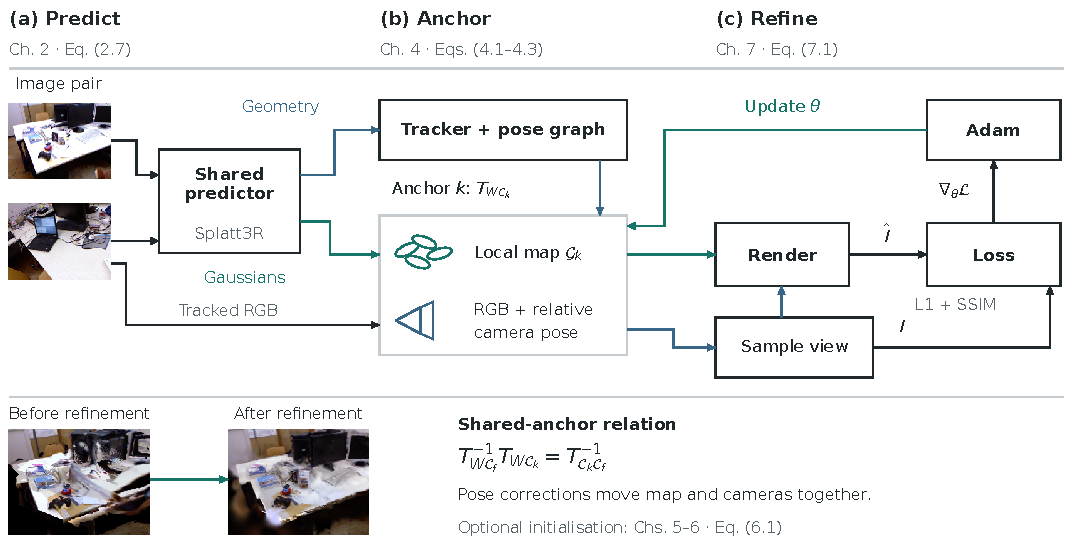
\includegraphics[width=\linewidth]{ral/fig/method_overview_master.pdf}
  \caption[Predict, anchor, and refine]{Method navigation. Real input frames
  enter a shared predictor. Geometry feeds tracking, while local Gaussians
  attach to keyframe anchors. The same anchors carry supervision cameras.
  A separate process samples observations, renders the map, and updates its
  appearance. Chapter and
  equation labels point to the detailed derivation.}
  \label{fig:method-overview}
\end{figure}

The refiner runs in its own process. This allows it to use a different GPU,
which \cref{ch:refiner} shows reduces contention in the measured TUM desk
configuration.
It also separates photometric optimisation from geometric tracking: the
refiner reads the pose state but does not optimise or write tracking poses.
Resource contention can still affect scheduling and end-to-end throughput.

SharedKeyframes stores images, pointmaps, confidences, poses and Gaussian
payloads in CUDA tensors exposed through inter-process communication.
The refiner transfers new Gaussian payloads to its device and reads current
anchor poses. Separately, tracked RGB supervision and anchor-relative camera
transforms live in the CPU SupervisionFrames pool. Complete refined maps are
published through a CPU snapshot buffer. These are distinct storage paths.

\begin{figure}[t]
  \centering
  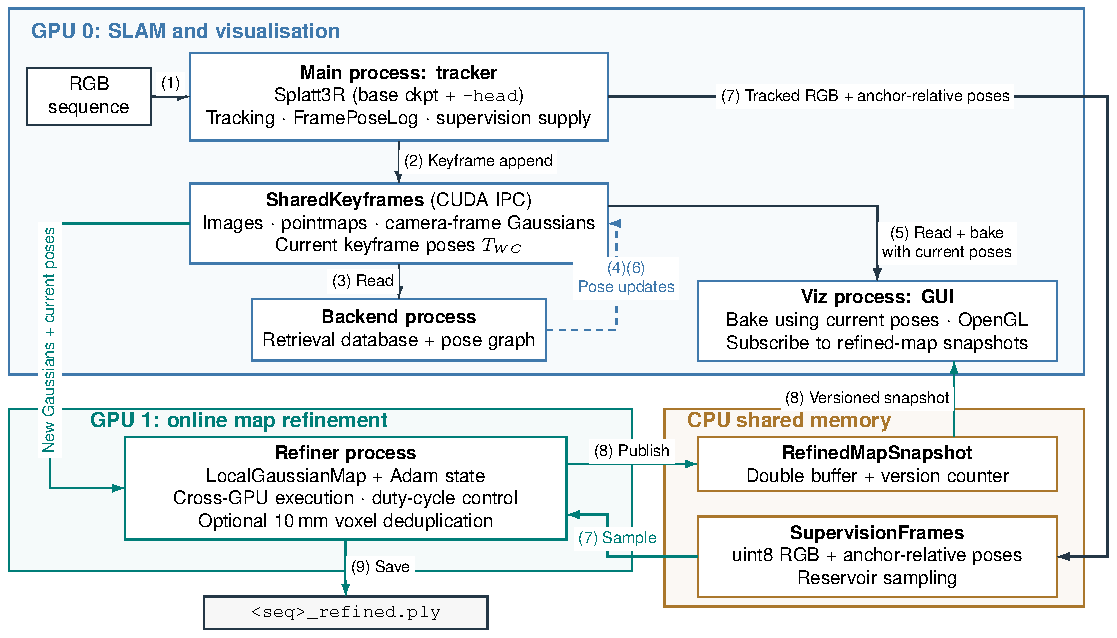
\includegraphics[width=\linewidth]{ral/fig/overview.pdf}
  \caption[System overview]{System overview.
  Tracking, backend optimisation, and visualisation run on GPU~0; the map
  refiner runs on GPU~1. SharedKeyframes uses CUDA IPC, while supervision
  frames and versioned refined-map snapshots use CPU shared memory.
  Numbered arrows show RGB, predicted pointmaps, local Gaussians, supervision
  and refined-map flow; dashed arrows denote pose updates. Thumbnails use
  real TUM desk predictions and recorded maps. Before/after renders share
  one camera; the backend inset shows recorded keyframe camera centres.}
  \label{fig:system-overview}
\end{figure}

\section{Anchor-carried map composition}
\label{sec:system:anchor}
We replace the pointmap prediction with Splatt3R, so each keyframe pair yields
a per-pixel Gaussian in one forward pass. Keyframe Gaussians are stored in
their anchor keyframe's local frame and composed into the world through that
keyframe's \emph{current} pose,
\begin{equation}
\mu_n^{W}=a_kR_k\mu_n^{\mathcal C_k}+t_k,\qquad
\Sigma_n^{W}=a_k^2R_k\Sigma_n^{\mathcal C_k}R_k^\top,
\label{eq:anchor}
\end{equation}
where $T_{W\mathcal C_k}=(a_kR_k,t_k)$ is the camera-to-world
$\mathrm{Sim}(3)$ pose of keyframe $k$. Because the composition reads the
pose at render time, a loop closure that updates $T_{W\mathcal C_k}$ moves
the map without rewriting local parameters.

Supervision uses the same anchor. If tracked frame $f$ stores a relative pose
$T_{\mathcal C_k\mathcal C_f}$, then
\begin{equation}
T_{W\mathcal C_f}
=T_{W\mathcal C_k}T_{\mathcal C_k\mathcal C_f}.
\label{eq:supervisionpose}
\end{equation}
For a local map and camera sharing anchor $k$, their relative transform is
\begin{equation}
T_{W\mathcal C_f}^{-1}T_{W\mathcal C_k}
=(T_{W\mathcal C_k}T_{\mathcal C_k\mathcal C_f})^{-1}
 T_{W\mathcal C_k}
=T_{\mathcal C_k\mathcal C_f}^{-1}.
\label{eq:anchorconsistency}
\end{equation}
The anchor cancels, so any invertible update of $T_{W\mathcal C_k}$ preserves
this relation. The identity applies within one anchor; neighbouring local maps
can still disagree.

The implementation stores means, scales, rotations, SH coefficients, opacity,
confidence, and validity in a shared keyframe buffer. Tracker updates may
rewrite pointmap state without clearing the Gaussian record unless a new
Gaussian prediction is present. This invariant prevents a geometric update
from silently erasing an already renderable keyframe. Filtering and the
global Gaussian limit are applied before rasterisation; the limit is therefore
a rendering budget implemented through spatial stride, rather than FIFO
deletion of individual keyframes.

\section{The injection pipeline}
\label{sec:system:injection}

Between ``the network emitted a Gaussian'' and ``the Gaussian is in the map''
sit several filters, and their order matters because two of them interact with
the contribution of \cref{ch:thin}.

\begin{enumerate}\itemsep3pt
\item \textbf{Validity.} Pixels without a valid pointmap prediction emit no
      Gaussian.
\item \textbf{Confidence gate.} Gaussians below \texttt{--refiner-min-confidence}
      are dropped outright. This is a \emph{deletion} operation and is
      deliberately kept distinct from thinning, which is not.
\item \textbf{Scale clamp.} An optional cap on injected scale, applied at
      refinement time and independent of the bake-time cap, bounds the damage a
      single mispredicted $\hat{s}$ can do to a render.
\item \textbf{Band-limiting.} Injected Gaussians are optionally band-limited
      against the measured lattice pitch of the prediction grid
      (\texttt{--refiner-aa-sigma}), which removes the dot/moir\'e pattern that
      a per-pixel Gaussian field otherwise produces when viewed off-axis.
\item \textbf{Opacity thinning.} \Cref{eq:thin}, the subject of
      \cref{ch:thin}.
\end{enumerate}

The global Gaussian limit is applied \emph{before} rasterisation and is
implemented as a spatial stride over the map, not as FIFO deletion of
keyframes. The distinction is not cosmetic: a FIFO policy would make the
displayed map a function of how long the sequence has been running, whereas a
stride makes it a function of the display budget alone, and leaves the
evaluation artefact --- the full map, written to disk --- untouched by whatever
the viewer could afford to draw.

\section{Rendering, display and the evaluation artefact}
\label{sec:system:render}

The refiner publishes a versioned snapshot in CPU memory rather than exposing
mutable GPU state. The visualiser uploads only complete versions and retains
the previous valid version if it collides with a write. If the display buffer
is smaller than the refined map, publication subsamples --- but only after the
full map has been saved. This ordering means a failure to publish a large map
for display cannot discard a valid refinement result, which is a failure mode
we hit before separating the two paths.

On termination the system writes the refined map as a standard 3DGS
\texttt{.ply}, so that it can be scored, inspected or rendered by any tool in
that ecosystem rather than only by ours. The external rendering comparisons
in \cref{ch:results} use these artefacts and the full-SH evaluation script.
Earlier component ablations use the recorded map-scoring harness for their
respective paired runs. Neither uses viewer screenshots as quantitative data.

\section{Changes to MASt3R-SLAM}
\label{sec:system:diff}

We replace the pointmap
prediction with Splatt3R's joint pointmap-and-Gaussian prediction; we add the
Gaussian record to the shared keyframe buffer; we add the injection pipeline
of \cref{sec:system:injection}; and we add the refiner process of
\cref{ch:refiner}. We change nothing in matching (\cref{eq:trackray}), nothing
in keyframe selection, nothing in the retrieval path, and nothing in the
back-end solver (\cref{eq:global}).

The one place where this could leak is the pointmap itself, since Splatt3R and
MASt3R share an encoder and decoder but the fine-tuned head is ours. Head-only
training (\cref{ch:adapt}) keeps the encoder and decoder bit-frozen, so the
pointmap the tracker consumes is bit-identical to what MASt3R would have
produced. This is why \cref{sec:exp:ate} reports parity rather than
improvement; it serves as a control for the inherited tracking path.

\chapter{Adapting the Feed-Forward Head}
\label{ch:adapt}

\section{Choosing the trainable module}
\label{sec:method:head}

Splatt3R trains its Gaussian head against frozen encoder and decoder features.
We compare three adaptation choices:

\begin{itemize}\itemsep2pt
\item \textbf{Encoder LoRA}~\cite{hu2022lora} ($r{=}8$, $\alpha{=}16$ on
      \texttt{qkv}/\texttt{proj}/\texttt{fc1}/\texttt{fc2}):
      $-49\%$ reconstruction quality against the released checkpoint, with
      predicted scales exploding by $1821\times$. The failure is immediate,
      not a late-training instability.
\item \textbf{Decoder-only LoRA}: $+0.37$\dB{} at epoch~1, then collapse to
      $-1.61$\dB{} by epoch~5 with a $12\times$ climb in the $99$th-percentile
      scale.
\item \textbf{Head-only} (encoder and decoder bit-frozen, only
      \texttt{gaussian\_dpt} trainable): improves, and is what we keep.
\end{itemize}

The collapse coincides with the exponential Gaussian-scale parameter
$s_n=\exp(\hat{s}_n)$. A small feature shift can produce a large scale change,
while different scale--opacity combinations can fit the same supervision
views. We therefore retain head-only training for the evaluated system.
The shared encoder, decoder, and geometric heads remain frozen; the Gaussian
DPT head uses the upstream objective and Adam~\cite{kingma2015adam}.

\section{Training setup}
\label{sec:adapt:setup}

Adaptation is performed per dataset family. The families differ in sensor,
exposure, motion, and depth availability. Each receives its own head
checkpoint, loaded at start-up.

The objective is the upstream one of \cref{eq:splatt3rloss}, unchanged, so
that the comparison against the released checkpoint isolates the data and the
choice of what to train, not the loss. Only \texttt{gaussian\_dpt} receives
gradients; the encoder and decoder are frozen, and this is verified by
comparing parameter hashes before and after training rather than by trusting
a \texttt{requires\_grad} flag.

The TUM, EuRoC and 7-Scenes heads in the reported paired adaptation study
were trained for $40$ epochs. Their batch sizes are $2$, $4$ and $8$, with
learning rates $10^{-5}$, $1.41\times10^{-5}$ and $2\times10^{-5}$,
respectively. A $15\%$ validation split is drawn within the available family
data. These experiments measure in-family adaptation; they do not establish
transfer to an unseen dataset family or a sequence-disjoint benchmark.

Two of the five families (EuRoC and ETH3D) ship no usable depth for the
training pairs. Rather than exclude them, pairs are supervised with
self-predicted pseudo-depth from the frozen backbone. This is a weaker
supervision signal, and the results in \cref{ch:results} should be read with
that in mind: EuRoC is the family where the refiner contributes least
($+1.00$\dB) and ETH3D the family where it contributes most ($+8.69$\dB),
and we do not have an explanation for that spread
(\cref{sec:neg:attrib}).

\section{Photometric augmentation and the opacity channel}
\label{sec:adapt:aug}

\Cref{sec:method:mech} examines opacity's photometric role. Inputs darkened
independently of target views provide a controlled way to test whether
opacity statistics respond to appearance perturbations. The SH residual
can also change colour, so this experiment does not isolate opacity as the
only compensating channel.

Four augmentation regimes were trained for $40$ epochs each on the same family
and probed with an identical five-pair protocol. The table reports the
$90$th-percentile predicted scale (a proxy for how far the head has moved from
the released checkpoint's geometry), the median predicted opacity, and the
fraction of Gaussians with opacity above $0.9$ --- i.e.\ how saturated the
opacity channel is:

\begin{center}
\small
\begin{tabular}{@{}lrrrr@{}}
\toprule
Head & scale p90 & inflation & median $\alpha$ & $\alpha>0.9$ \\
\midrule
base (released)              & \phantom{0}9.78 & ---       & 1.000 & 100.0\% \\
content noise + blur         & 26.18 & $+167.8\%$ & 1.000 & 100.0\% \\
global photometry            & 17.37 & $+77.6\%$  & 0.991 & \phantom{0}83.1\% \\
spatial photometry           & 14.82 & $+51.5\%$  & 0.876 & \phantom{0}42.9\% \\
content + spatial photometry & 10.97 & $+12.2\%$  & 0.933 & \phantom{0}62.7\% \\
\bottomrule
\end{tabular}
\end{center}

Three things are visible. The released checkpoint's opacity is
\emph{completely saturated} --- median $1.000$, every Gaussian above $0.9$ ---
which provides little initial differentiation between primitives and
motivates testing an external attenuation prior. Content-only
augmentation does not move the channel at all while inflating scale by
$168\%$. Global photometry modestly reduces saturation; spatial photometry
reduces it much more strongly, from $100\%$ to $42.9\%$. These are observed
parameter responses, rather than a complete account of what the head learned.

The combined regime was tested against an explicit prediction: if the two
perturbations engage independently, saturation should fall to $30$--$50\%$
\emph{and} scale inflation should exceed $10\%$. Scale inflation cleared the
bar at $+12.2\%$, barely; saturation landed at $62.7\%$, \emph{above} the
predicted range and above what spatial photometry achieved on its own. Both
numbers moved in the direction of mutual suppression rather than independent
engagement. The prediction is therefore not supported.

Across four scenes the spatial-photometry
head gives a mean LPIPS improvement of $-14.55\%$, with a per-scene spread of
$-6.6\%$ to $-19.2\%$. The gain is scene-dependent.

\chapter{Injection-Time Thinning and the Opacity Mechanism}
\label{ch:thin}

\section{The crowding problem}
\label{sec:thin:crowding}

A two-view prediction covers each visible surface once. A SLAM map covers it
once \emph{per keyframe that saw it}, and on a typical indoor sequence that is
tens of times. Nothing in the pipeline reconciles these copies: each is
predicted independently, placed by its own keyframe's pose, and injected with
whatever opacity its forward pass produced.

Under \cref{eq:alphacomp} the consequence is specific rather than generic. If
the copies agreed in colour and depth, stacking would still change effective
opacity: $K$ copies with opacity $\alpha$ have combined opacity
$1-(1-\alpha)^K$. Inconsistent copies additionally differ in depth by the per-forward scale gauge
(\cref{sec:neg:frontend} measures this at ${\sim}5\%$), in colour by the
source-frame photometric anchoring of \cref{eq:colorresidual}, and in extent by
the head's own scale prediction. A ray therefore accumulates opacity from
several slightly-displaced, slightly-different surfaces before its
transmittance runs out, and what should be one sharp surface composites into
haze.

The released checkpoint makes this worse in a way that is visible in its
statistics rather than in its images: its predicted opacity is
\emph{saturated}, with median $1.000$ and every Gaussian above $0.9$
(\cref{sec:adapt:aug}). A saturated opacity channel cannot express ``this
copy should contribute less''. The lever below supplies that expression from
outside the network.

\section{Insertion-time opacity attenuation}
\label{sec:thin:lever}
\label{sec:method:thin}

A SLAM map covers each surface with predictions from many keyframes. Under
\cref{eq:alphacomp} with a black background, a surface covered by many
over-solid Gaussians composites to haze rather than to a sharper surface. We
therefore fade opacity at the moment a Gaussian enters the map, in proportion
to how little the pointmap confidence vouches for it.

Confidences are not calibrated across keyframes, so we rank-normalise
\emph{within} each keyframe. For a keyframe with $N$ Gaussians and confidence
values $\{c_n\}$, let $r_n$ be the rank of $c_n$ and
$\hat{c}_n = r_n/(N-1) \in [0,1]$. The injected opacity is
\begin{equation}
\alpha'_n \;=\; \alpha_n \cdot
\mathrm{clip}\Bigl(1 - 2\lambda\,(1-\hat{c}_n),\; 0.1,\; 1\Bigr),
\label{eq:thin}
\end{equation}
with dose $\lambda{=}0.45$ in the thinning experiments. External comparisons
disable thinning with $\lambda=0$. The lower clip at $0.1$ retains every
primitive and its refinement gradient.

\subsection{Relation to pairwise training}
An opacity penalty added to \cref{eq:splatt3rloss} would act during pair
training. Crowding appears later, after SLAM accumulates
keyframes over a surface, and \cref{eq:splatt3rloss} never sees more than two
context views. Consistent with this, we measured that the refiner
un-saturates opacity on its own even with the released head (median
$1.0\rightarrow0.26$). Attenuation therefore starts the map closer to an
opacity state that the optimiser can reach. A dose--response check at two
thinning depths (opacity knees $0.9$ and $0.6$) gave $-21.0\%$ and
$-15.8\%$ LPIPS. Benefits persist for these heads, supporting complementarity
in this experiment. A different training objective or sequence-level
training procedure might still learn an equivalent adjustment.

\section{Opacity, colour, and visibility}
\label{sec:method:mech}

The DC colour is an SH residual added to the encoding of input RGB, with
clamping at conversion (\cref{eq:colorresidual}). Both the residual and
opacity can respond to photometric perturbations. Opacity additionally
controls which surfaces remain visible along a ray.

For an isolated primitive over black, greater opacity increases its
contribution. In a multicolour stack it may instead obscure brighter content.
The background therefore does not imply a monotone relation between opacity
and brightness. We test their correlation without assigning a unique cause.

We registered a sign-specific prediction. Let $\ell$ be input
luminance and $\rho$ the Spearman correlation between $\alpha$ and $\ell$ over
predicted Gaussians. A head trained with independently darkened inputs
(synthetic vignetting and white-balance jitter) was predicted to have
$\rho<0$, whereas a real-sensor head without synthetic darkening was
predicted to have $\rho>0$. \Cref{sec:exp:mech} reports both signs in the
five tested heads: two Replica augmentation heads and three real-data
heads. These are five models, not five independent dataset families.
Correlations are consistent with opacity responding to photometry, but do
not identify a unique causal mechanism.

\section{Controls}
\label{sec:thin:ablations}

\subsection{Confidence weighting}

\Cref{eq:thin} fades in proportion to rank-normalised confidence, and the name
``confidence-weighted thinning'' invites the reading that the confidence signal
is what makes it work. We measured the alternative --- the same total dose
applied \emph{uniformly}, with no confidence term at all --- and against
confidence weighting it is statistically a coin flip: $n{=}12$ online cells,
median difference $-0.06\%$.

Reducing injected opacity is the robust effect in this study. The
confidence-weighted form concentrates reduction where the pointmap is least
sure, but the uniform control performs similarly.

\subsection{Shape-weighted attenuation}

A second opacity lever reduces each Gaussian's opacity in proportion to how
elongated it is relative to its local surface sampling. It targets trailing
primitives near depth discontinuities. In measurement it fades $64$--$98\%$
of all Gaussians by $39$--$65\%$ of their opacity. Its effect is therefore
broad rather than sparse.

LPIPS improves on the three tested sequences by $-12.7\%$, $-6.6\%$, and
$-1.3\%$, with a PSNR change of $-0.04$ to $-0.22$\dB{}.
The LPIPS gain is largest in scenes with more streaked geometry.

\chapter{Online Map Refinement}
\label{ch:refiner}

\section{Design}
\label{sec:method:refiner}

Prediction supplies an initialisation. A separate process photometrically
refines the assembled map \emph{while SLAM runs}; together with the GUI,
the complete system has four processes (\cref{fig:overview}).

\subsection{Parameterisation}
Gaussians are optimised in their anchor keyframe's local frame in
pre-activation form --- $\log s$, unnormalised $q$, $\mathrm{logit}\,\alpha$,
and the SH DC term --- so that scales stay positive and opacity stays in
$(0,1)$ without constraints, and composed to the world by
\cref{eq:anchor} at every step. Per-group Adam rates follow the 3DGS
reference, with the positional rate scaled by scene extent:
$\eta_\mu = 1.6\!\times\!10^{-4}\!\cdot\!\mathrm{extent}$,
$\eta_{f_{dc}} = 2.5\!\times\!10^{-3}$, $\eta_\alpha = 5\!\times\!10^{-2}$,
$\eta_s = 5\!\times\!10^{-3}$, $\eta_q = 1\!\times\!10^{-3}$.

\subsection{Objective}
Supervision views are tracked frames, so the refiner optimises
\begin{equation}
\mathcal{L}_{\text{ref}} = (1-\lambda_{D})\,\lVert \hat{I}-I \rVert_1
                          + \lambda_{D}\,\bigl(1-\mathrm{SSIM}(\hat{I},I)\bigr),
\qquad \lambda_{D}=0.2 ,
\label{eq:refloss}
\end{equation}
i.e.\ the 3DGS objective rather than \cref{eq:splatt3rloss}: LPIPS is a
reporting metric here, not a training signal, so that our evaluation metric is
not also our loss.

\subsection{Anchor-carried supervision}
Each supervision frame is stored as an image together with
$(\text{anchor index}, T_{\text{anchor},f})$ rather than a world pose. Its
world pose is recomposed through the anchor's \emph{current} pose at sample
time, so supervision follows loop closures exactly as the map does under
\cref{eq:anchor,eq:supervisionpose}. Frames are held in CPU shared memory,
which allows the refiner to run on a second GPU.
The refiner consequently never becomes a second pose-graph writer: a loop
closure changes the anchor pose once, and both map placement and supervision
views follow that correction.

\subsection{Sampling}
Supervision is drawn from a reservoir of $200$ frames spanning the whole
sequence plus a ring of the $64$ most recent, with a recent fraction of $0.3$.
We measured uniform-over-history to dominate a recency-weighted schedule
(held-out early/late split: $14.40/14.09/14.72$ uniform versus
$14.06/13.79/14.35$ recent-only), because causal arrival already biases the
pool toward recent views.

\subsection{Scheduling}
Sharing one GPU, the refiner holds a duty cycle $d$ by sleeping
$\mathrm{EMA}[\Delta t]\,(1-d)/d$ after each step, so optimisation steps are
dropped but never frames. Refiner load on the \emph{same} card doubles tracker
latency ($101\!\rightarrow\!206$\,ms p50); on a second card it is noise
($103$\,ms), which is the configuration we deploy. After the sequence ends an
optional polish phase continues with the final poses.

\subsection{Centre updates}
The external-comparison configuration holds $\mu$ fixed. Earlier fixed-map
experiments also favoured this choice at approximately $300$ and $3000$
steps. The broader causal delivery study did not show the same preference.
External comparisons and causal studies therefore report their centre
settings separately from the command-line defaults in \cref{app:hyper}.

When centres are fixed, the positional learning rate above is inactive.
When enabled, centre updates can trade geometric consistency against fit
to supervision cameras. \Cref{sec:exp:online} separates the tested causal
configuration from the fixed-centre, post-sequence comparison.

The refiner publishes a versioned CPU snapshot rather than mutable GPU state.
The visualiser uploads only complete versions and retains the previous valid
version on a read/write collision. If the display buffer is smaller than the
refined map, publication subsamples after the full map has been saved. This
separates bounded display memory from the evaluation artifact and prevents a
large-map publication failure from discarding a valid refinement result.

\section{The polish phase}
\label{sec:refiner:polish}

When the sequence ends, the trajectory stops changing but the map is still
under-optimised: every step taken during the sequence was taken against poses
that were still moving. A \emph{polish} phase continues refinement with the
final poses, and it is the single largest online win we measured:
$+2.21$\dB{} PSNR and $-16.7\%$ LPIPS over seven TUM \texttt{fr1} sequences.

The required duration varies. Sequences need
between $1445$ and $3821$ steps to converge --- a $2.6\times$ spread --- and no
static quantity we tried predicts which sequence needs which: not length, not
keyframe count, not final Gaussian count, not the loss at the start of the
phase. A fixed step budget therefore either wastes time on the easy sequences
or truncates the hard ones. The implementation offers a convergence
criterion (\texttt{--refiner-polish-tol} with a patience of two logging
windows), disabled by default. Its stopping rule and fixed-duration
experiments should be reported separately.

\Cref{tab:tum} uses a fixed $300$\,s budget for our external comparison,
rather than convergence-based stopping. Its PSNR is close to MonoGS after
$339$\,s colour refinement, while MonoGS has lower LPIPS. A separate
historical $1200$\,s run reached $14.61$\,dB and $0.379$ LPIPS under the
older evaluation configuration. That experiment demonstrates further
optimisation headroom; it is not mixed into the fresh full-SH comparison or
presented as a gain at matched total compute.

\section{Density control}
\label{sec:refiner:omissions}

The refiner reinstates the 3DGS objective (\cref{eq:3dgsloss}) but not the
adaptive density control that accompanies it in the reference implementation.
This choice has a measurable map-size cost.

Cloning and splitting are omitted because the map already has an excess of
primitives rather than a shortage: the failure mode this thesis addresses is
crowding, and a densification policy tuned for a sparse SfM initialisation
would be solving the opposite problem. Pruning and periodic opacity reset
are also omitted. Pruning changes the primitive count and requires
corresponding updates to optimiser and snapshot state. Opacity reset changes
the optimisation schedule.

The cost is visible in \cref{sec:lim:compact}: without pruning, nothing ever
removes a primitive that the data does not support, and the map size is
whatever the injection pipeline produced. A voxel-based deduplication pass was
implemented as a partial substitute and measured as a negative: it removes
$27.6\%$ of the map for $-0.53$\dB{}. We report it as a map-size control that
costs quality when it fires without a recovery budget, and it is off by
default. Refining directly under a primitive budget --- rather than pruning
after the fact --- is the future work named in \cref{ch:conclusion}.

\section{Tracking preservation}
\label{sec:refiner:invariant}

The refiner reads and composes poses through
\cref{eq:anchor,eq:supervisionpose}, without optimising them. The recorded
ablations preserve ATE ($0.016975$\,m, rounding to the $0.0170$\,m baseline)
while changing map quality by several dB. This supports the intended
separation of mapping and tracking. It does not eliminate resource contention
or guarantee identical scheduling in every multi-process run.

\chapter{Evaluation Protocol}
\label{ch:protocol}

All comparison maps and trajectories come from local runs on a host with two
RTX~A6000 GPUs. This chapter defines the common full-SH renderer, cameras,
alignment, and aggregation.

\begin{table}[htbp]
\centering
\small
\setlength{\tabcolsep}{4pt}
\begin{tabular}{@{}llcl@{}}
\toprule
System & Type & Rend. & Role here \\
\midrule
Ours & mono 3DGS & \checkmark & --- \\
Photo-SLAM & mono 3DGS & \checkmark & rendering \\
MonoGS & mono 3DGS & \checkmark & rendering (TUM) \\
MASt3R-SLAM & mono dense & --- & tracking control \\
VGGT-SLAM & pose+cloud & --- & tracking control \\
\bottomrule
\end{tabular}
\caption[Systems compared, and what each can produce]{Systems compared: Photo-SLAM~\cite{huang2024photoslam},
MonoGS~\cite{matsuki2024monogs}, MASt3R-SLAM~\cite{murai2025mast3rslam},
VGGT-SLAM~\cite{maggio2025vggtslam}. The latter two supply trajectory
comparisons only; MASt3R-SLAM is the inherited tracking control.}
\label{tab:systems}
\end{table}


\section{Common rendering conditions}

For each scene, $100$ frames are selected outside the union of participating
systems' keyframes. Each exported map is rendered at these same cameras by
one implementation, with identical exposure normalisation and metric code.
The resolution is $512\times288$ on Replica and $512\times384$ on TUM.
All exported spherical-harmonic bands are retained: degree three for
Photo-SLAM, degree zero for the evaluated MonoGS and our maps.

Scene PSNR is computed as $-10\log_{10}$ of the mean frame MSE, rather than
as the arithmetic mean of per-frame PSNR. LPIPS-AlexNet~\cite{zhang2018lpips}
is averaged across frames. Dataset means weight each scene equally.
Scene PSNR and the median paired frame difference can therefore rank methods
differently.

\subsection{Evaluation scope}

We call these \emph{non-keyframe reconstruction} scores. Tracked
non-keyframes may enter the refiner's supervision pool. Their exclusion from
the keyframe set therefore does not guarantee they were unseen during
optimisation. Ground-truth cameras reduce dependence on each system's own
evaluation-pose estimates, but expose tracking and alignment errors as well
as map errors. Common rendering also cannot remove differences in input
preprocessing, undistortion or optimisation history.

A strict novel-view experiment would exclude scoring views from every
optimisation and model-selection path.

\subsection{Datasets and configurations}

Rendering covers all eight Replica~\cite{straub2019replica} scenes and TUM
RGB-D~\cite{sturm2012tum} \texttt{freiburg1\_desk}, with monocular input for
all compared systems. Trajectory accuracy covers all nine TUM freiburg1
sequences. Adaptation and refinement studies additionally use
EuRoC~\cite{burri2016euroc}, ETH3D~\cite{schops2017eth3d} and
7-Scenes~\cite{shotton2013scenecoord}.

The external rendering configuration uses the released Splatt3R head,
fixed Gaussian centres, insertion thinning disabled and $300$\,s
post-sequence refinement. Photo-SLAM runs to its own shutdown schedule, so
Replica optimisation budgets are not matched. MonoGS uses a $339$\,s
colour-refinement phase on TUM desk. That phase is close in duration to our
polish, but is not a match of total pipeline compute.

Family-head adaptation and thinning use separate paired runs. Maps delivered
at sequence end are reported separately from post-sequence polish.

\subsection{Alignment}

Each monocular map has its own similarity gauge. We fit a map-to-ground-truth
alignment $(s,R,t)$ to corresponding estimated and ground-truth camera centres
using Umeyama's method~\cite{umeyama1991}. A ground-truth camera-to-world pose
is transported into map coordinates by
\begin{equation}
R_{\text{map}}=R^\top R_{\text{gt}},\qquad
t_{\text{map}}=R^\top(t_{\text{gt}}-t)/s.
\label{eq:align}
\end{equation}
The inverse scale acts on translation, not on the rotation block. Putting it
inside the rotation would produce a non-orthonormal camera orientation.
ATE is translation RMSE after similarity alignment, evaluated with
\texttt{evo\_ape tum -as}~\cite{grupp2017evo}.

MonoGS records estimated and ground-truth keyframe poses together. Its TUM
keyframes are recovered from those saved GT poses and checked against GT
orientation. This avoids confusing indices in its RGB-D-associated stream
with indices in the raw RGB sequence. The updated comparison uses this
association throughout selection, alignment and rendering.

\section{Self-consistency and provenance}
\label{sec:protocol:selfcheck}

Before interpreting a cross-system margin, the exported map is rendered at
the poses from which it was built. A poor result here requires checking
camera conventions, image association and map loading before interpreting
it as a property of the method. In an earlier MonoGS diagnostic, interpreting
camera-to-world poses as world-to-camera changed the measured score from
$18.71$ to $4.36$\,dB. Those are diagnostic values from that experiment,
not the updated common-camera scores in \cref{tab:tum}.

The current evidence records the input PLY and trajectory hashes and sizes,
alignment transforms, all scoring frame indices, per-frame metrics and
representative-view selection. It also records DC-only scores for comparison
with the older renderer, which discarded higher SH bands. The updated
Photo-SLAM Replica mean is $19.483$\,dB with full SH, compared with
$19.581$\,dB in that DC-only evaluation. The external tables use full SH
consistently; historical ablations retain their original configurations.

Qualitative views are selected at the two middle ranks of the per-frame
Ours-minus-baseline PSNR difference: MonoGS on TUM and Photo-SLAM on Replica.
All methods receive the same crop coordinates and image scale. This makes
selection repeatable without selecting the most favourable tail.

\section{Pose-source sensitivity}
\label{sec:protocol:offset}

Earlier diagnostics rendered an unchanged MonoGS map from its estimated
poses and from aligned ground-truth poses, obtaining $18.71$ and
$9.87$\,dB, respectively. A separate Photo-SLAM diagnostic measured a
smaller difference of approximately $2.6$\,dB. These experiments demonstrate
that map quality is coupled to the camera poses used to evaluate it.
They also include alignment error and the degree to which map parameters
have adapted to their training cameras.

An earlier local-to-published comparison changed views, resolution, masking,
undistortion, and optimisation budget at once. It cannot isolate a fixed
protocol offset. The comparison tables therefore contain only locally
rendered scores under the conditions above.

\section{Systems compared}
\label{sec:protocol:systems}

\Cref{tab:systems} identifies each system's available outputs.
We did not obtain a monocular MonoGS Replica map with the available
configurations; its depth-assisted configuration is excluded.

Comparable three-method TUM artefacts were obtained on desk; broader
rendering coverage remains future work. Photo-SLAM uses OpenCV~4.10 for
CUDA compatibility rather than its tested 4.7/4.8 stack.
\Cref{app:baselines} records this preprocessing-related deviation.

\chapter{Results}
\label{ch:results}

This chapter moves from component studies to the complete system.
The external comparison uses the full-SH protocol of \cref{ch:protocol}.

\section{Head-only adaptation}
\label{sec:exp:head}

Family heads are evaluated on assembled maps as well as on validation pairs.
The paired deployment study holds refinement active and disables thinning
in both arms. Improvements vary across scenes and families: ETH3D reports
$-29.1\%$ LPIPS, EuRoC $-20.8\%$, and four TUM sequences range from
$-7.9\%$ to $-25.9\%$. Replica adaptation is also beneficial in its
recorded study, whereas 7-Scenes is weak and ranges from a $0.14\%$ increase
to a $4.9\%$ decrease in LPIPS. These results do not imply that every
family or sequence benefits.

\begin{table}[t]
\centering\small
\begin{tabular}{@{}llrr@{}}
\toprule
Family & Sequence & $\Delta$PSNR (dB) & Relative $\Delta$LPIPS \\
\midrule
EuRoC & MH\_01 & $+0.62$ & $-20.8\%$ \\
TUM & desk & --- & $-7.9\%$ \\
TUM & room & --- & $-9.9\%$ \\
7-Scenes & chess & $+0.10$ & $+0.14\%$ \\
\bottomrule
\end{tabular}
\caption[Paired head-adaptation examples]{Family head versus released head,
with refinement enabled and thinning disabled in both arms. A dash denotes
a PSNR difference not tabulated here. Negative relative LPIPS is better.
These are separate adaptation runs, not the external-comparison maps.}
\label{tab:head}
\end{table}

A two-head, two-seed check gives relative differences below $5\%$ with
inconsistent signs at validation and deployment. Training uses an in-family
validation split.

\subsection{Tested explanations}
The variation in gains remains unexplained. \Cref{tab:falsified} records
four proposed explanations and the measurements that contradicted them.
The recorded $0.17\%$ LPIPS variation applies to those paired probes.

\begin{table}[t]
\centering\small
\setlength{\tabcolsep}{3pt}
\begin{tabular}{@{}p{0.30\linewidth}p{0.62\linewidth}@{}}
\toprule
Candidate & Why it fails \\
\midrule
Scale-frame consistency &
Mechanically inert: \cref{eq:splatt3rloss} is purely photometric, means are
\texttt{detach()}ed, and the metric-scale flag's only consumer is disabled.
Depth touches training solely via the mask. \\
Supervision coverage &
Measured per family: EuRoC has the \emph{lowest} coverage ($39.5\%$) and the
second-largest gain; ETH3D matches TUM's coverage ($61.9$ vs $60.0\%$) with
$3\times$ the gain. \\
Opacity un-saturation &
Explains four families in rank order but 7-Scenes measures $0.479$ ---
comparable to EuRoC's $0.38$ --- with a null gain. A measured counterexample,
not a pending cell. \\
Base-checkpoint headroom &
$\rho=0.145$ over $11$ sequences. ETH3D \texttt{sofa\_1} has the lowest
deficit of any sequence and the second-largest gain. \\
\bottomrule
\end{tabular}
\caption[Four falsified attributions]{Four pre-registered mechanisms for the cross-family variation, each
killed by measurement. The variation is real and remains unattributed.}
\label{tab:falsified}
\end{table}


\section{Injection-time thinning}
\label{sec:exp:thin}

Across twelve online comparisons spanning four datasets, six heads and
eight scenes, ten cells improve LPIPS clearly and two are near zero. The
worst measured change is a $0.16\%$ increase. Confidence-weighted versus
uniform allocation has a median difference of only $-0.06\%$, with its
interval spanning zero. The evidence supports opacity attenuation more
strongly than this particular allocation rule.

\begin{table}[t]
\centering\small
\begin{tabular}{@{}llr@{}}
\toprule
Scene & Head & Relative $\Delta$LPIPS \\
\midrule
Replica office3 & Plain adapted & $-12.7\%$\\
Replica office0 & Plain adapted & $-12.6\%$\\
Replica office2 & Plain adapted & $-10.2\%$\\
Replica room0 & Plain adapted & $-8.9\%$\\
Replica room1 & Plain adapted & $-7.1\%$\\
Replica office1 & Plain adapted & $-1.6\%$\\
Replica office0 & Opacity knee 0.9 & $-5.3\%$\\
Replica office0 & Opacity knee 0.6 & $-1.8\%$\\
TUM desk & Released & $-6.4\%$\\
TUM desk & Adapted & $-0.6\%$\\
EuRoC MH\_01 & Adapted & $-5.6\%$\\
7-Scenes chess & Adapted & $+0.16\%$\\
\bottomrule
\end{tabular}
\caption[Fine-grained opacity attenuation ablation]{Relative LPIPS change
for confidence-ranked attenuation with $\lambda=0.45$ versus off.
Refinement is active in both arms. Negative values improve LPIPS.}
\label{tab:thinning}
\end{table}


\subsection{Dose--response}
Two tested opacity regimes yield thinning gains of $-21.0\%$ and
$-15.8\%$ LPIPS. Without thinning, refinement itself changes median opacity
from approximately $1.0$ to $0.26$ in a released-head TUM map.
These findings show that insertion starts the map closer to an opacity state
that refinement can reach.

\section{Opacity and input luminance}
\label{sec:exp:mech}

\Cref{tab:lum} reports the registered sign test. The two Replica heads
trained with synthetic darkening have negative opacity--luminance
correlations; the three real-data heads have positive correlations.
All five tested heads match the predicted sign. The set contains two Replica
augmentation heads and three real-data heads. The SH residual and visibility
can also affect the correlation.

\begin{table}[t]
\centering\small
\begin{tabular}{@{}llr@{}}
\toprule
Head & Training data & $\rho(\alpha,\text{luminance})$ \\
\midrule
photospatial & Replica + synthetic darkening & $-0.316$ \\
mixed        & Replica + synthetic darkening & $-0.279$ \\
TUM          & real sensor                   & $+0.303$ \\
ETH3D        & real sensor                   & $+0.392$ \\
EuRoC        & real sensor                   & $+0.304$ \\
\bottomrule
\end{tabular}
\caption[Opacity--luminance correlations on five heads]{Registered
opposite-sign prediction, matched by five tested heads: two Replica
augmentation heads and three real-data heads. This correlation experiment
does not establish a unique causal interpretation of opacity.}
\label{tab:lum}
\end{table}


\section{Rendering: Replica, all eight scenes}
\label{sec:exp:replica}

\Cref{tab:replica} compares monocular maps from the released head with
fixed centres, thinning disabled and $300$\,s polish against Photo-SLAM.
Our mean is $23.019$\,dB versus $19.483$\,dB, a $3.536$\,dB difference.
PSNR is higher on all eight scenes. Mean LPIPS is $0.135$ versus $0.163$,
with improvements on five scenes; Photo-SLAM is better on office2,
office4 and room2. PSNR differences range from $0.23$\,dB on room1 to
$7.64$\,dB on room0. Replica optimisation budgets are not matched.

\begin{table}[t]
\centering\small
\setlength{\tabcolsep}{3.5pt}
\begin{tabular}{@{}lrrrr@{}}
\toprule
& \multicolumn{2}{c}{PSNR (dB) \up} & \multicolumn{2}{c}{LPIPS \dn}\\
Scene & Photo-SLAM & Ours & Photo-SLAM & Ours\\
\midrule
office0 & 22.19 & \textbf{26.30} & 0.219 & \textbf{0.104} \\
office1 & 17.77 & \textbf{22.08} & 0.190 & \textbf{0.115} \\
office2 & 20.15 & \textbf{20.97} & \textbf{0.135} & 0.150 \\
office3 & 19.20 & \textbf{20.18} & 0.165 & \textbf{0.144} \\
office4 & 16.43 & \textbf{23.65} & \textbf{0.129} & 0.156 \\
room0 & 17.81 & \textbf{25.44} & 0.159 & \textbf{0.110} \\
room1 & 21.68 & \textbf{21.91} & 0.181 & \textbf{0.139} \\
room2 & 20.64 & \textbf{23.62} & \textbf{0.123} & 0.160 \\
\midrule
Mean & 19.48 & \textbf{23.02} & 0.163 & \textbf{0.135} \\
\bottomrule
\end{tabular}

\caption[Rendering on Replica, all eight scenes]{Replica reconstruction
with monocular input and full exported SH. Bold identifies the better value
per scene and metric. Ours uses the released head, fixed centres, no thinning
and 300\,s polish. PSNR improves on eight scenes and LPIPS on five;
optimisation budgets and primitive counts differ.}
\label{tab:replica}
\end{table}


\begin{figure}[t]
  \centering
  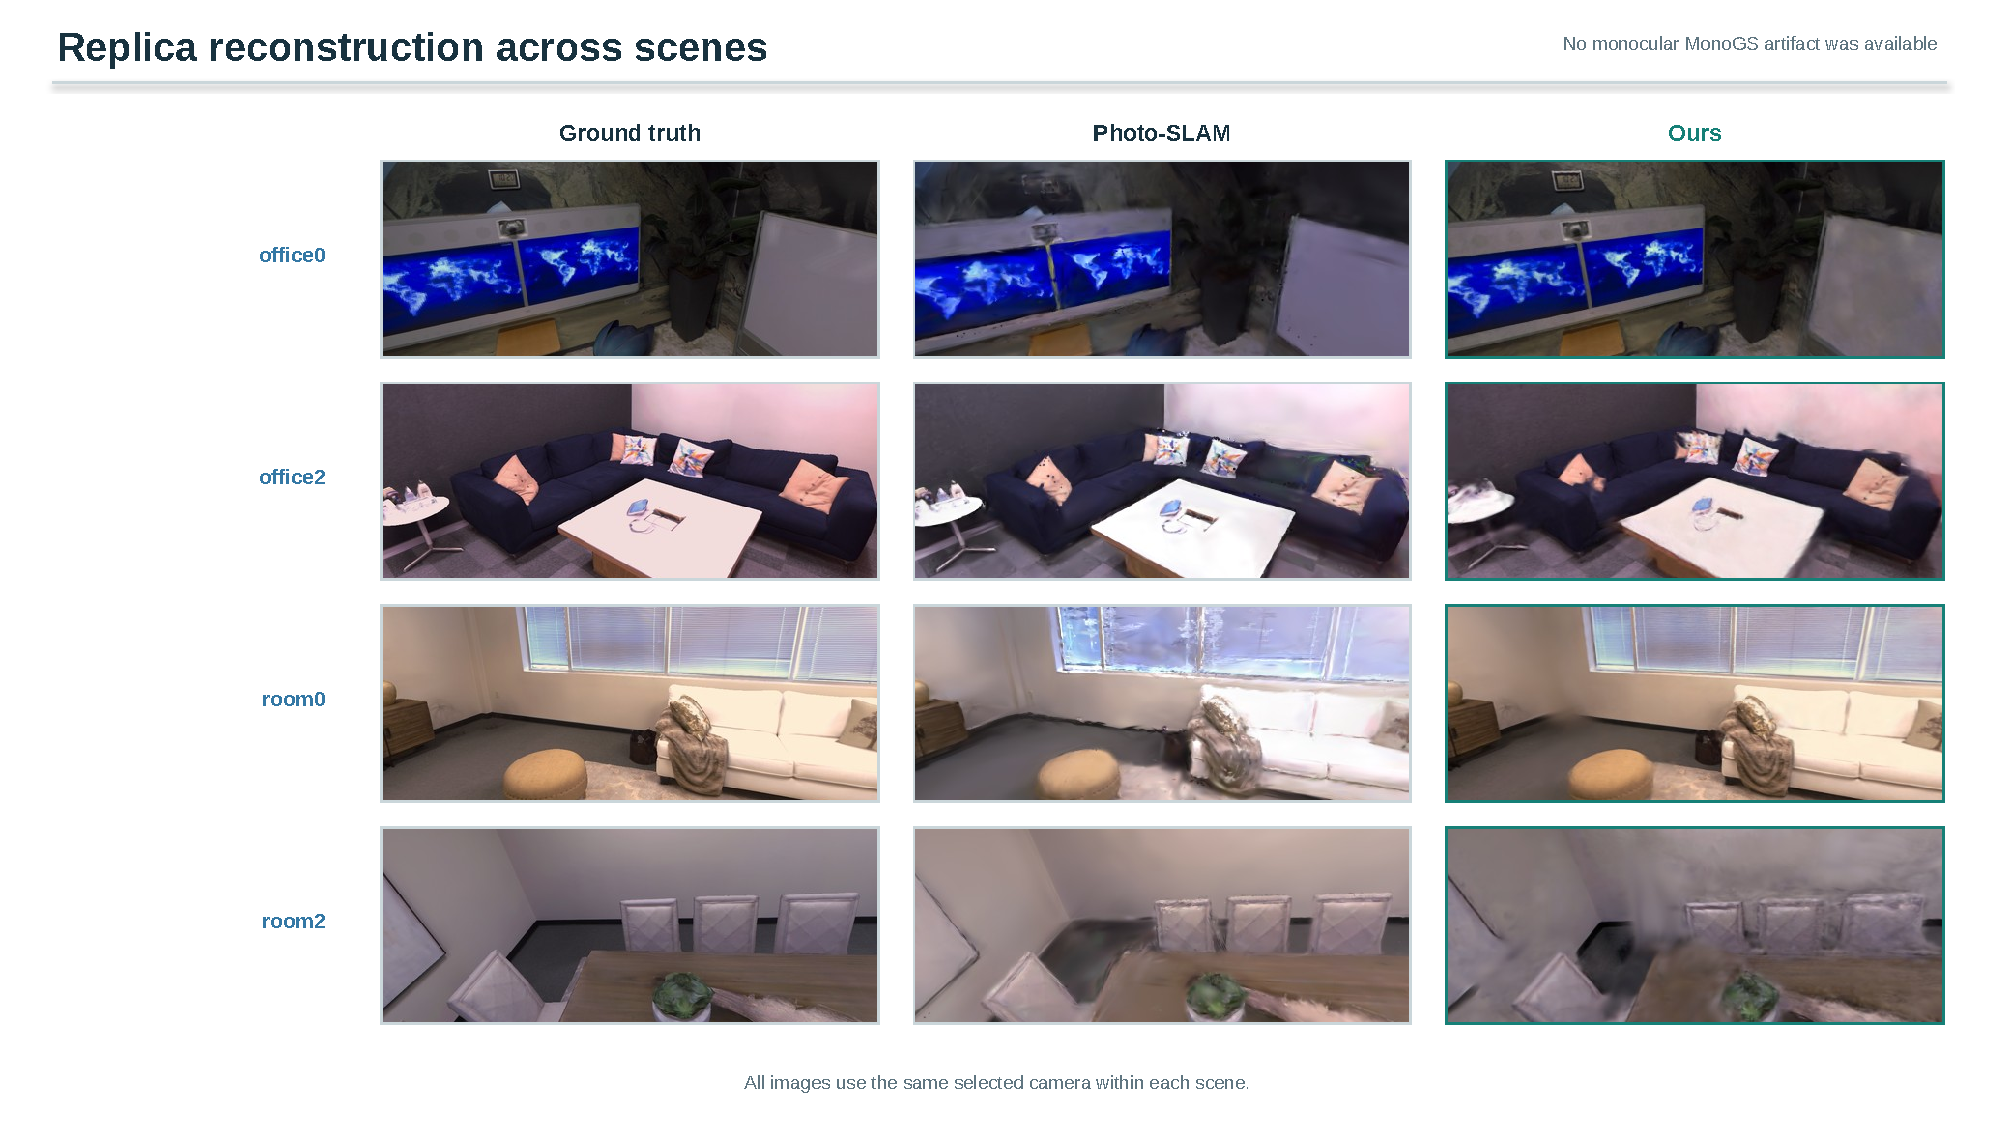
\includegraphics[width=\linewidth]{ral/fig/qualitative-replica.pdf}
  \caption[Replica qualitative comparison]{Ground truth, Photo-SLAM, and
  Splatt3R-SLAM on four Replica scenes. Each row uses one common evaluation
  camera. MonoGS is absent because no comparable monocular Replica map was
  available.}
  \label{fig:qualitative-replica}
\end{figure}

\begin{figure}[t]
  \centering
  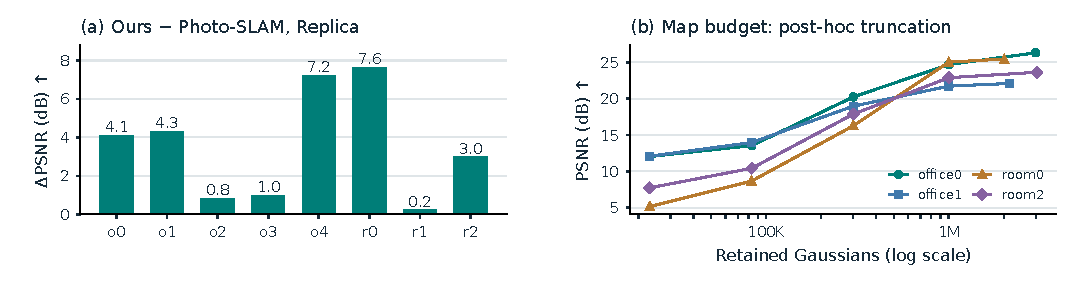
\includegraphics[width=\linewidth]{ral/fig/evidence.pdf}
  \caption[Scene dependence and map truncation]{(a) Fresh full-SH Replica
  scene PSNR differences; o/r denote office/room. (b) A separate recorded
  experiment retaining the highest-opacity primitives in four of our maps,
  without re-optimisation. Final markers denote full maps. The truncation
  curve measures sensitivity to this procedure, not optimal quality under
  each primitive budget.}
  \label{fig:evidence}
\end{figure}

\subsection{Scene aggregates and per-frame distributions}

A scene score aggregates MSE before taking the logarithm. It need not rank
methods like the median of per-frame PSNR differences.
\Cref{tab:frame-distribution} derives both statistics from the same $100$
frames used in each fresh comparison. On office2 and room1 the scene
difference is positive but the median frame difference is negative, and our
method wins only $42$ and $38$ frames, respectively.
On room0 the median difference is $+7.498$\,dB, but Photo-SLAM still has
the higher PSNR on $24$ frames.

\begin{table}[t]
  \centering\small
  \begin{tabular}{@{}lrrr@{}}
\toprule
Scene & Scene $\Delta$PSNR & Frame median & Positive frames\\
\midrule
office0 & +4.115 & +3.543 & 100/100 \\
office1 & +4.312 & +3.041 & 87/100 \\
office2 & +0.822 & -1.124 & 42/100 \\
office3 & +0.977 & +0.058 & 51/100 \\
office4 & +7.215 & +5.826 & 77/100 \\
room0 & +7.637 & +7.498 & 76/100 \\
room1 & +0.230 & -0.697 & 38/100 \\
room2 & +2.983 & +3.294 & 73/100 \\
TUM desk & +0.035 & -0.411 & 41/100 \\
\bottomrule
\end{tabular}

  \caption[Per-frame PSNR differences]{Ours minus Photo-SLAM on Replica,
  and Ours minus MonoGS on TUM desk. Scene $\Delta$PSNR uses each method's
  mean frame MSE; frame median uses paired per-frame PSNR differences.
  Positive frames counts strict numerical wins.}
  \label{tab:frame-distribution}
\end{table}

Representative images use the two middle ranks of these paired differences.
The office0 teaser and TUM qualitative figure therefore show typical
differences under a reproducible selection rule, rather than the largest
positive margins.

\section{Rendering: TUM desk and optimisation budget}
\label{sec:exp:tum}

\Cref{tab:tum} reports $13.949$\,dB for our map and $13.914$\,dB for
MonoGS. MonoGS has lower LPIPS,
$0.395$ versus $0.411$. Both exceed Photo-SLAM under this protocol.
Our $300$\,s polish and MonoGS's $339$\,s colour refinement are close in
duration, but total pipeline costs differ. This three-method rendering
comparison covers one TUM sequence.

\begin{table}[t]
\centering\small
\setlength{\tabcolsep}{4pt}
\begin{tabular}{@{}lrrr@{}}
\toprule
Method & PSNR (dB) \up & LPIPS \dn & $N$ (thousands)\\
\midrule
Photo-SLAM & 10.67 & 0.562 & 36.1 \\
MonoGS & 13.91 & 0.395 & 23.0 \\
Ours & 13.95 & 0.411 & 2396.9 \\
\bottomrule
\end{tabular}

\caption[Rendering on TUM \texttt{fr1\_desk}]{TUM desk reconstruction at
common cameras, retaining full exported SH. Ours uses 300\,s polish and
MonoGS 339\,s colour refinement; total pipeline compute is not matched.
$N$ counts exported primitives. This three-method rendering comparison
covers one sequence.}
\label{tab:tum}
\end{table}


\begin{figure}[t]
  \centering
  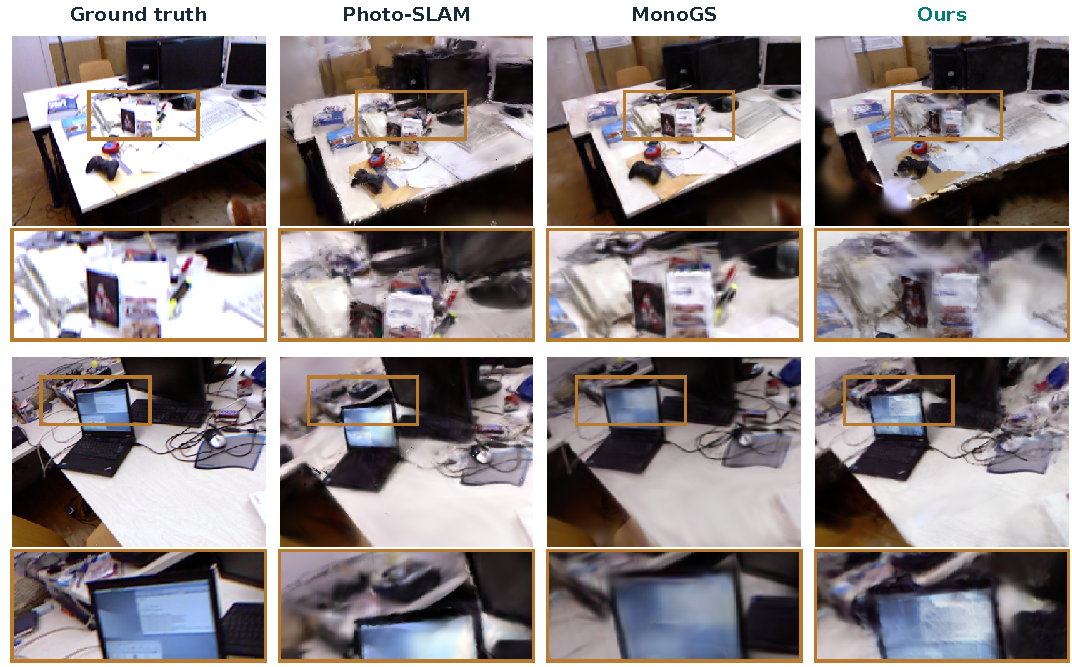
\includegraphics[width=\linewidth]{ral/fig/qualitative_tum.pdf}
  \caption[Four-column TUM reconstruction comparison]{Ground truth,
  Photo-SLAM, MonoGS and Ours, at two common TUM desk cameras. Each full
  view is followed by an identical crop, indicated in orange. Views occupy
  the two middle ranks of Ours-minus-MonoGS per-frame PSNR. Remaining blur
  and geometric distortion are visible in both MonoGS and our maps.
  No per-image score labels are used.}
  \label{fig:qualitative}
\end{figure}

Only $41$ of the $100$ TUM frames have higher PSNR for our method than
MonoGS, and the median difference is $-0.411$\,dB. This complements the
close scene aggregate and cautions against treating it as uniform visual
superiority. A separate historical $1200$\,s polish experiment reached
$14.61$\,dB and $0.379$ LPIPS under its original scoring configuration;
it measures additional-budget behaviour and is not a row in the fresh
common-budget comparison.

\section{Trajectory accuracy}
\label{sec:exp:ate}

\Cref{tab:ate} reports all nine TUM sequences. Our mean ATE is essentially
the same as MASt3R-SLAM's, consistent with preserving its geometric path.
This is a tracking-preservation control rather than a new tracking result.
Photo-SLAM is most accurate on several sequences but has large errors on
desk2, room and teddy. MonoGS also has large errors on several runs, which
strongly influence its mean. Multi-threaded tracking is not deterministic:
two Photo-SLAM desk runs yielded $0.0174$ and $0.0149$\,m ATE.

\begin{table}[t]
\centering\small
\setlength{\tabcolsep}{3pt}
\begin{tabular}{@{}lrrrrr@{}}
\toprule
Seq. & Ours & MASt3R & VGGT & Photo & MonoGS \\
\midrule
360   & 0.042 & 0.048 & 0.050 & \best{0.035} & 0.177 \\
desk  & 0.017 & 0.016 & 0.025 & \best{0.015} & 0.036 \\
desk2 & 0.028 & \best{0.024} & 0.029 & 0.438 & 0.844 \\
floor & 0.027 & 0.025 & 0.099 & \best{0.013} & 0.539 \\
plant & \best{0.015} & 0.020 & 0.025 & 0.046 & 0.071 \\
room  & \best{0.059} & 0.061 & 0.064 & 0.510 & 0.791 \\
rpy   & \best{0.022} & 0.023 & 0.026 & 0.057 & 0.041 \\
teddy & 0.048 & 0.045 & \best{0.036} & 0.305 & 0.123 \\
xyz   & \best{0.009} & \best{0.009} & 0.014 & 0.010 & 0.017 \\
\midrule
Mean  & \best{0.030} & \best{0.030} & 0.041 & 0.161 & 0.293 \\
\bottomrule
\end{tabular}
\caption[Trajectory accuracy, TUM freiburg1, five systems]{ATE RMSE (m), TUM freiburg1, all nine sequences and all five systems.
Photo-SLAM is non-deterministic (ORB-SLAM3 is multi-threaded): \texttt{desk}
gave $0.0174$ and $0.0149$ on two runs, so its single-run figures carry
run-to-run variance.}
\label{tab:ate}
\end{table}


\section{Shared anchors and refinement}
\label{sec:exp:refiner}

\subsection{Pose-correction control}
A blockwise $\mathrm{Sim}(3)$ test applies a 6\% scale correction to saved
TUM desk and room anchors. With fixed world-space supervision cameras,
refinement largely reverses the correction after about 500 steps. With
anchor-carried supervision, it is retained. This controlled test supports
the coordinate relation in \cref{eq:anchorconsistency}.

\subsection{Refinement on and off}
\Cref{tab:refiner} separates several recorded refinement interventions.
Holding the released head fixed and toggling refinement with $300$\,s
polish gives $+8.69$\,dB on ETH3D sofa\_1, $+4.62$\,dB on Replica
office0, $+3.52$\,dB on TUM desk and $+1.00$\,dB on EuRoC V1\_01.
Their relative LPIPS improvements are $58.3\%$, $56.8\%$, $27.3\%$
and $14.5\%$. These are not instantaneous online gains.

\begin{table}[t]
\centering\small
\setlength{\tabcolsep}{4pt}
\begin{tabular}{@{}lrl@{}}
\toprule
Ablation & $\Delta$PSNR & Note \\
\midrule
Refiner on, ETH3D   & $+8.69$ & 300\,s polish \\
Refiner on, Replica & $+4.62$ & \\
Refiner on, TUM     & $+3.52$ & \\
Refiner on, EuRoC   & $+1.00$ & \\
\midrule
Causal replay, 120 it. & $+1.21$ & TUM desk \\
Second GPU, unthrottled & $+2.15$ & tracker 101 to 103\,ms \\
\midrule
Uniform vs.\ recency & $+0.34$ & held-out mean \\
Voxel dedup, 10\,mm & $-0.53$ & $-27.6\%$ map size \\
\bottomrule
\end{tabular}
\caption[Refinement ablations]{Refinement ablations. ATE is unchanged in every row
($0.016975$ vs.\ a $0.0170$ baseline in the deterministic configuration): the
map is strictly downstream of tracking, and the pre-registered failure
condition ``ATE moves at all'' never fired. Earlier fixed-map probes favoured
freezing centres at approximately 300 and 3000 steps; the broader causal study
did not support making this a universal online default. The dedup row is a map-size
control that costs quality when it fires without a recovery budget, not a
quality feature.}
\label{tab:refiner}
\end{table}


\section{Online delivery across dataset families}
\label{sec:exp:online}

The deployed path is measured separately with family heads, causal SLAM,
the GUI enabled and refinement on a second GPU. \Cref{tab:online} reports
quality before polish. Seven of nine sequences improve LPIPS; TUM room and
360 worsen it by $11.1\%$ and $20.6\%$, despite small PSNR gains.
The refiner does not write pose corrections.

\begin{table}[t]
\centering\small
\setlength{\tabcolsep}{2.7pt}
\begin{tabular}{@{}llrrrr@{}}
\toprule
Family & Sequence & Bake P & Refine P & $\Delta$P & $\Delta$L \\
\midrule
TUM & desk & 12.42 & 13.75 & +1.33 & $-7.5\%$ \\
TUM & room & 11.15 & 11.45 & +0.30 & $+11.1\%$ \\
TUM & 360 & 12.00 & 12.14 & +0.14 & $+20.6\%$ \\
7-Scenes & chess & 13.44 & 13.79 & +0.35 & $-4.8\%$ \\
7-Scenes & office & 11.64 & 11.74 & +0.10 & $-1.6\%$ \\
7-Scenes & pumpkin & 14.15 & 14.91 & +0.77 & $-4.1\%$ \\
EuRoC & MH\_01 & 10.17 & 11.67 & +1.50 & $-4.1\%$ \\
EuRoC & V1\_01 & 12.06 & 12.69 & +0.63 & $-13.0\%$ \\
ETH3D & plant\_1 & 20.42 & 22.22 & +1.80 & $-7.4\%$ \\
\bottomrule
\end{tabular}
\caption[Online delivery, GUI on, dual GPU]{Actual GUI-on, dual-GPU online delivery. P is PSNR in dB and L is
LPIPS; $\Delta L$ is relative, so negative is better. Seven of nine cells
improve LPIPS. TUM room and 360 gain a little PSNR but lose perceptual quality
under the in-sequence budget, exposing supervision starvation on their large
maps rather than a universal refiner improvement. ETH3D \texttt{cables\_1} is
omitted because its $0.5$-m scene and $0.1165$-m ATE make held-out rendering
alignment-dominated. The reported online values are from the pre-polish
delivery pass; the longer polish diagnostic is separated below.}
\label{tab:online}
\end{table}


Across these runs, refinement adds approximately $7$--$10\%$ frame time
with the GUI open. The head-only arm uses $19.8$--$39.6$~GB on GPU~0;
refinement adds $1$--$1.5$~GB there and uses $2.8$--$14.0$~GB on GPU~1.
The largest observed combination is $41.1$~GB plus $14.0$~GB.
The focused desk latency result therefore does not imply negligible
overhead throughout the broader campaign.

\subsection{Budget and centre-update diagnostics}

\begin{table}[t]
\centering\small
\begin{tabular}{@{}lrrrr@{}}
\toprule
Iterations & 120 & 500 & 1000 & 3000\\
\midrule
Causal PSNR & 13.651 & 14.394 & 14.475 & 14.412\\
Post-hoc PSNR & 13.800 & 14.322 & 14.352 & 14.375\\
\bottomrule
\end{tabular}
\caption[Refinement iteration-budget control]{TUM desk PSNR in the recorded
causal and post-hoc replay. Both arms use the same map-evaluation protocol.}
\label{tab:budget}
\end{table}


The iteration control in \cref{tab:budget} shows that most of the TUM desk
gain appears by 500 steps. Additional causal iterations do not improve
monotonically. In the broader campaign, the deployed desk/360/room maps
received only $104/114/190$ refinement
steps; post-sequence polish supplied $1581/3821/1856$ steps and improved
PSNR by $+1.97/+2.30/+2.22$\,dB and LPIPS by $-22.0/-8.3/-15.9\%$.
An offline proxy suggested a position-learning-rate explanation for the
online degradation, but the causal loop did not reproduce it.
The offline centre-freezing and band-limit choices did not supply a
general online fix. Optimisation budget and coverage are the main measured
differences between the short causal and long polish phases.

\section{System cost}
\label{sec:exp:cost}

\Cref{tab:cost} compares recorded TUM desk costs with the same GPU memory
sampler. Our refiner-off run takes $70$\,s and peaks at $21{,}035$\,MiB;
Photo-SLAM takes $28$\,s and $1{,}286$\,MiB. These costs do not include
our $300$\,s polish.
Our exported desk map has $2.397$ million primitives, against $36{,}069$
for Photo-SLAM and $23{,}019$ for MonoGS.

\begin{table}[t]
\centering\small
\setlength{\tabcolsep}{5pt}
\begin{tabular}{@{}lrrl@{}}
\toprule
System & Wall clock \dn & Peak GPU (MiB) \dn & Note \\
\midrule
Ours        & \phantom{0}70\,s & 21{,}035 & $6.47$\,fps, refiner off \\
Photo-SLAM  & \best{\phantom{0}28\,s} & \best{\phantom{0}1{,}286} & fastest and leanest \\
MonoGS      & 555\,s & \phantom{0}2{,}389 & $404$\,s of it optimisation \\
VGGT-SLAM   & \phantom{0}24\,s & \phantom{0}9{,}436 & no renderable map \\
\bottomrule
\end{tabular}
\caption[System cost, all four systems]{End-to-end cost on TUM
\texttt{fr1\_desk} ($613$ frames), one GPU held exclusively for the
measurement, the same $1$\,Hz sampler for every system. VGGT-SLAM's time is
not comparable to the other three in what it buys: it produces poses and a
point cloud, not a renderable map. Our peak memory is $16\times$
Photo-SLAM's and $8.8\times$ MonoGS's, and Photo-SLAM is $2.5\times$ faster
end-to-end. Our row has refinement disabled and does not include the
post-sequence polish used in the external rendering comparison.}
\label{tab:cost}
\end{table}


The dense per-pixel representation is one source of this cost, alongside
model, optimiser and rendering storage. Naive opacity-ranked truncation
degrades reconstruction sharply (\cref{tab:curve}). It motivates
direct optimisation under a primitive budget. \Cref{app:tables} gives
per-family costs and extended truncation measurements.

\chapter{Negative Results}
\label{ch:negative}

Several interventions improved an intermediate metric but harmed the complete
SLAM system. This chapter records those tests because they narrow the design
space and explain choices made in earlier chapters.

\section{Backbone adaptation}
\label{sec:neg:lora}

Encoder LoRA~\cite{hu2022lora} was tested as a broader alternative to
head-only adaptation. Reconstruction quality fell by $49\%$ and predicted
Gaussian scales increased by $1821\times$. Decoder-only LoRA improved by
$0.37$\dB{} after one epoch, then fell to $-1.61$\dB{} by epoch five while
the 99th-percentile scale increased by $12\times$.

Both failures combine a feature change with an exponentially parameterised
scale head. The measured signature motivates the frozen-backbone design in
\cref{ch:adapt}. It applies to the tested objectives and regularisation;
other joint adaptation methods remain open.

\section{Independent multi-pair averaging}
\label{sec:neg:aggregation}

One way to reduce pairwise scale variation is to predict a new keyframe
against several partners, align their depth scales, and average the maps.
With $m\in\{1,2,4,8\}$ predictions, scale disagreement falls from $5.16\%$
to $3.06\%$. A single sixteen-view VGGT forward reaches $1.68\%$.
Independent averaging reduces random variation but cannot impose one shared
scale across all views. It also requires $m$ forward passes per keyframe.

\section{Loop-closure retrieval refitting}
\label{sec:neg:retrieval}

The inherited retrieval system uses a PCA transform and an ASMK codebook.
A $2048$-centroid refit on $279$ TUM keyframes improves weighted offline
Recall@1 by $20\%$. End-to-end SLAM gives a different result:
\texttt{room} ATE improves by $8.2\%$, \texttt{360} degrades by $24.1\%$,
and \texttt{desk} degrades by $318.8\%$ to near the no-loop-closure control.
The evaluated system therefore retains the original MASt3R retrieval assets.
Candidate recall alone does not measure the effect of accepted edges on the
pose graph.

\section{Cross-family adaptation variation}
\label{sec:neg:attrib}

Head-only adaptation gains vary across datasets. Four explanations were
tested: residual mismatch, base-quality headroom, novelty to the training
corpus, and sensor modality. Each conflicts with at least one paired result
in \cref{tab:falsified}. The available evidence therefore reports the
variation without assigning one cause.

\section{Geometric scale correction}
\label{sec:neg:frontend}

Pairwise pointmaps show per-keyframe scale variation. We tested whether a
many-view model could estimate better local scales and whether those scales
would improve the Gaussian map.

\subsection{Context and backbone}
The gauge-free scale spread in \cref{tab:scale} separates model choice from
view context. The same VGGT~\cite{wang2025vggt} weights give $10.82\%$ spread
when run pairwise and $1.68\%$ when sixteen views enter one forward pass.
The two-view MASt3R control gives $5.16\%$. Multi-view context, rather than
the backbone alone, produces the lower spread.

\begin{table}[t]
\centering\small
\setlength{\tabcolsep}{5pt}
\begin{tabular}{@{}llrr@{}}
\toprule
Predictor & Context & Views & Disagreement \dn \\
\midrule
Splatt3R (deployed) & pairwise & 2 & $5.35\%$ \\
VGGT~\cite{wang2025vggt} & pairwise & 2 & $10.82\%$ \\
VGGT~\cite{wang2025vggt} & joint & 16 & \best{$1.68\%$} \\
\midrule
\multicolumn{4}{@{}l}{\emph{disjoint-window replication}} \\
Splatt3R & pairwise & 2 & $4.92\%$ \\
VGGT & joint & \phantom{0}8 & \best{$1.53\%$} \\
\bottomrule
\end{tabular}
\caption[Adjacent-view depth-scale disagreement]{Adjacent-view depth-scale disagreement, gauge-free, TUM freiburg1,
pooled over seven sequences ($84$ windows above the rule, $33$ disjoint
windows below it). Windows in the primary arm overlap by $80$--$97\%$, so the
result is replicated on eight-view windows tiled by exactly one span; the
replication is $7/7$ sequences, paired Wilcoxon $p=8.6\times10^{-8}$. VGGT's
$1.68\%$ sits at or below the RGB-D sensor's own view-dependent bias floor, so
it is a lower bound on how far coupling goes.}
\label{tab:scale}
\end{table}


\subsection{Map edit}
A sixteen-view estimate supplies one scale correction per keyframe cluster.
On TUM desk, sensor-referenced scale error improves from $6.48\%$ to
$1.02\%$. Rendering becomes worse: PSNR falls from $12.35$ to
$11.50$\dB{} and LPIPS rises from $0.507$ to $0.523$.
After $300$\,s refinement, PSNR changes from $13.81$ to $13.08$\dB{}.
The same trend appears on \texttt{360} and \texttt{room}.

\subsection{Scale prior during refinement}
Using the correction as a prior instead of a fixed edit also reduces image
quality. As prior weight rises from $0.05$ to $0.5$, PSNR falls from
$13.74$ to $13.38$\dB{} and LPIPS rises from $0.449$ to $0.456$.
The fitted scale spread remains $2.6\%$, compared with the reference
correction of $8.0\%$.

These tests show a conflict between isolated scale accuracy and the current
photometric map fit. Camera poses, local geometry, and appearance have been
estimated together; editing one part can reduce their internal agreement.
A prior explanation based on a $0.057$\,m keyframe baseline was withdrawn
after contribution-weighted rendering rays showed a baseline near $0.78$\,m.
The negative result rests on the measured edits and priors, not on that
earlier explanation.

\section{Result of the negative studies}
\label{sec:neg:method}

The failed routes improve reconstruction loss, retrieval recall, or local
scale accuracy without improving the final map or trajectory. For this
system, an intervention is retained only when its end-to-end metric improves
under the target execution path. This rule leads to three concrete choices:
freeze shared features, keep the inherited retrieval assets, and avoid
map-only scale correction.

\chapter{Discussion and Limitations}
\label{ch:discussion}

\section{What shared anchors solve}

Shared anchors preserve the relative coordinates between a local Gaussian
map and the cameras used to refine it. The controlled pose-correction test
supports this relation, and trajectory accuracy remains close to the
MASt3R-SLAM control. This separation allows appearance refinement to run in
another process without becoming a second pose optimiser.

The construction does not merge neighbouring local maps. Two anchors can
still predict different depths, colours, or extents for the same surface.
Seams and cross-frame colour changes can therefore remain after loop closure.
Joint optimisation of poses, geometry, and appearance is a possible extension.

\section{Map size}
\label{sec:lim:compact}

Dense prediction creates substantially more primitives than the compared
systems. On Replica, our count is about $22.5$--$42.5$ times Photo-SLAM's.
On TUM desk, the ratios are about $66$ to Photo-SLAM and $104$ to MonoGS.
The refiner-off desk run uses $16.4$ times Photo-SLAM's peak GPU memory.

\Cref{tab:curve} keeps the highest-opacity primitives at smaller budgets and
re-renders without optimisation.

\begin{table}[t]
\centering\small
\setlength{\tabcolsep}{4pt}
\begin{tabular}{@{}lrrrr@{}}
\toprule
Gaussians kept & office0 & office1 & room0 & room2 \\
\midrule
full ($\sim$2--3M)     & 26.29 & 22.08 & 25.44 & 23.62 \\
1{,}000{,}000          & 24.68 & 21.71 & 25.01 & 22.87 \\
300{,}000              & 20.23 & 18.96 & 16.26 & 17.87 \\
83{,}372               & 13.54 & 13.97 & \phantom{0}8.68 & 10.43 \\
23{,}019               & 12.04 & 12.08 & \phantom{0}5.16 & \phantom{0}7.74 \\
\bottomrule
\end{tabular}
\caption[PSNR versus map budget, four Replica scenes]{Separate recorded
truncation study on our maps. Highest-opacity primitives are retained
without re-optimisation. Quality remains closer to the full map around one
million primitives and declines sharply at smaller budgets. These points
are not an estimate of optimal quality when trained or refined at each budget.}
\label{tab:curve}
\end{table}


Quality falls sharply below about one million primitives in this test.
The result shows that opacity-ranked removal after full-map optimisation is
insufficient. It does not measure a map trained under the smaller budget.
Budget-aware insertion, merging, pruning, and refinement are therefore
important next steps.

\section{Online refinement}

Moving refinement to a second GPU keeps median tracking latency close to the
refiner-off control on TUM desk. The broader campaign still uses up to
$41.1$~GB on GPU~0 and $14.0$~GB on GPU~1. Seven of nine maps improve LPIPS
before polish, while two larger TUM maps worsen.

The iteration study explains part of this gap. Most of the TUM desk gain
appears by 500 steps, but maps in the causal campaign receive only
$104$--$190$ steps before sequence end. A fixed compute budget supplies fewer
updates per region as the map grows. Adaptive region and view scheduling
should therefore be evaluated together with latency and memory.

\section{Evaluation scope}

The Replica comparison covers eight scenes; the three-method TUM rendering
comparison covers desk. All maps are rendered at common cameras, but input
preprocessing, map size, and total optimisation differ. Photo-SLAM runs to
its own shutdown schedule on Replica. On TUM, our $300$\,s polish is close
to MonoGS's $339$\,s colour phase, but does not equal total compute.

The scoring set excludes keyframes. Other tracked frames may still supervise
our refiner, so this is non-keyframe reconstruction rather than strict
unseen-view evaluation. A stronger generalisation experiment would exclude
scoring frames from every optimisation and model-selection path.

\section{Statistical coverage}

Several reported margins come from one run per configuration. The large
Replica PSNR difference is consistent across all eight scenes, while the
TUM PSNR difference to MonoGS is only $0.035$\,dB and the LPIPS ordering is
reversed. Confidence-ranked and uniform opacity attenuation are also close.
Repeated runs, more sequences, and matched resource budgets are needed to
resolve these smaller effects.

\chapter{Conclusion and Future Work}
\label{ch:conclusion}

This thesis asks how pairwise Gaussian predictions can become a persistent
SLAM map. Splatt3R-SLAM answers with shared keyframe anchors. Local Gaussians
and their supervision cameras follow the same pose corrections, while a
separate process improves appearance. The design keeps geometric tracking
inside MASt3R-SLAM and makes prediction, insertion, and refinement distinct
experimental stages.

\section{Answers to the research questions}

\paragraph{RQ1: adapting prediction}
Training only the Gaussian head preserves the shared features used by
tracking. It improves several dataset families, although the gain is weak on
7-Scenes. The tested encoder and decoder LoRA routes destabilise Gaussian
scale and reduce reconstruction quality.

\paragraph{RQ2: inserting overlapping predictions}
Opacity attenuation improves LPIPS in ten of twelve recorded comparisons.
Confidence-ranked allocation performs similarly to uniform attenuation, so
the main measured effect is the lower initial opacity. Refinement later moves
the median opacity in the same direction.

\paragraph{RQ3: sequence-level refinement}
Refinement improves PSNR by $1.00$--$8.69$\,dB in four on/off controls while
trajectory accuracy remains close to the inherited tracker. A second GPU
reduces contention in the desk control. Causal quality still depends on the
number and distribution of updates received before sequence end.

\paragraph{RQ4: complete-system comparison}
With the released head, no thinning, fixed centres, and $300$\,s polish,
Splatt3R-SLAM reaches $23.02$\,dB mean PSNR on eight Replica scenes,
compared with $19.48$\,dB for Photo-SLAM. It improves PSNR on all eight
scenes and LPIPS on five. On TUM desk, its $13.95$\,dB is close to
MonoGS's $13.91$\,dB, while MonoGS has lower LPIPS. These maps contain
millions of primitives and use much more memory than the compared systems.

\section{Future work}

The first priority is compact mapping. Primitive selection, merging, and
refinement should operate under a target memory budget instead of pruning a
full map after optimisation. The second is budget-aware online refinement:
view sampling and region scheduling should scale with map growth while
respecting a tracker-latency limit. The third is joint consistency across
anchors. Multi-view geometry, camera poses, and local appearance should be
updated together so that better geometry does not break an already fitted
rendering.

Evaluation should also expand beyond one TUM rendering sequence. Repeated
runs, matched total compute, sequence-disjoint adaptation, and a scoring set
excluded from all optimisation paths would separate small method differences
from execution variance. These steps would test whether dense pairwise
prediction can retain its reconstruction advantage in a compact, causal map.


\cleardoublepage
\phantomsection
\addcontentsline{toc}{chapter}{Bibliography}
\bibliographystyle{unsrtnat}
\bibliography{main}

\appendix
\chapter{Hyper-parameters and Configuration}
\label{app:hyper}

This appendix distinguishes current command-line defaults from settings
used in specific experiments. Historical ablations changed individual
options; no single default configuration describes every result.

\section{Head-only adaptation}

\begin{center}
\begin{tabular}{@{}lll@{}}
\toprule
Setting & Value & Note \\
\midrule
Trainable module   & \texttt{gaussian\_dpt} only & Gaussian prediction \\
Frozen             & encoder + decoder & checked unchanged \\
Objective          & \cref{eq:splatt3rloss} & upstream, unchanged \\
MSE weight         & $1.0$ & masked spatial average \\
VGG-LPIPS weight   & $0.25$ & masked spatial average \\
Optimiser          & Adam~\cite{kingma2015adam} & \\
Granularity        & one checkpoint per dataset family & \\
Families           & TUM, 7-Scenes, EuRoC, ETH3D, Replica & \\
\bottomrule
\end{tabular}
\end{center}

The two adaptation routes that were measured and rejected
(\cref{sec:neg:lora}) used LoRA rank $r{=}8$, $\alpha{=}16$ on
\texttt{qkv}/\texttt{proj}/\texttt{fc1}/\texttt{fc2}.

\section{Injection-time thinning}

\begin{center}
\begin{tabular}{@{}lll@{}}
\toprule
Flag & Default & Meaning \\
\midrule
\texttt{--refiner-conf-fade}    & $0.45$ & dose $\lambda$ of \cref{eq:thin} \\
\texttt{--refiner-uniform-fade} & $0$    & uniform-dose ablation arm \\
\texttt{--refiner-min-confidence} & $1.5$ & injection gate \\
lower clip                       & $0.1$ & thinning, not deletion \\
\bottomrule
\end{tabular}
\end{center}

All external-baseline comparisons in \cref{ch:results} were run with
\texttt{--refiner-conf-fade 0}, so the optional attenuation prior does not
contribute to our external-comparison result. Other systems use their own
mapping policies.

\section{Online refinement}

\begin{center}
\begin{tabular}{@{}lll@{}}
\toprule
Flag & Default & Measured setting \\
\midrule
\texttt{--refiner}              & off      & on \\
\texttt{--refiner-duty}         & $0.25$   & $1.0$ on a second GPU \\
\texttt{--refiner-gpu}          & $-1$     & $1$ (second card) \\
\texttt{--refiner-polish-secs}  & $0$      & $300$ \\
\texttt{--refiner-freeze-means} & on       & on in external comparison \\
\texttt{--refiner-aa-sigma}     & $0.5$    & regime-dependent \\
\texttt{--refiner-streak-opacity} & $0.5$  & \\
\texttt{--refiner-max-gaussians}& $4\,000\,000$ & dedup trigger \\
\texttt{--refiner-dedup-voxel}  & $0$      & $0.01$ measured, not shipped \\
\bottomrule
\end{tabular}
\end{center}

Learning rates, per group, follow the 3DGS reference with the positional rate
scaled by scene extent:
$\eta_\mu = 1.6\!\times\!10^{-4}\!\cdot\!\mathrm{extent}$,
$\eta_{f_{dc}} = 2.5\!\times\!10^{-3}$,
$\eta_\alpha = 5\!\times\!10^{-2}$,
$\eta_s = 5\!\times\!10^{-3}$,
$\eta_q = 1\!\times\!10^{-3}$.
The supervision reservoir holds $200$ frames spanning the sequence plus a ring
of the $64$ most recent, with recent fraction $0.3$.

\section{Hardware}

All numbers in this thesis were measured on a host with two NVIDIA RTX~A6000
GPUs. The single-GPU external cost campaign used an exclusively reserved
card and a common $1$\,Hz \texttt{nvidia-smi} sampler. The separate
GUI-enabled online campaign used both GPUs and reports their memory
separately. These measurements describe different experimental regimes.

\chapter{Reproduction}
\label{app:repro}

\section{Environment}

\begin{small}
\begin{verbatim}
git clone https://github.com/Looong01/Splatt3R-SLAM.git
cd Splatt3R-SLAM
conda create -n splatt3r-slam python=3.11 -y
conda activate splatt3r-slam
pip install torch torchvision --index-url \
    https://download.pytorch.org/whl/cu132
pip install cmake ninja swig mkl-devel
pip install -r requirements.txt
pip install -e thirdparty/in3d
pip install --no-build-isolation thirdparty/asmk
\end{verbatim}
\end{small}

\noindent
faiss is built from the vendored source with GPU support; the prebuilt PyPI
wheels must not be installed, because they shadow the build and pin
\texttt{numpy<2}:

\begin{small}
\begin{verbatim}
cd thirdparty/faiss
cmake -B build . && make -C build -j$(nproc) faiss swigfaiss
pip install --no-build-isolation --no-deps ./build/faiss/python
cd ../..
export CUDA_HOME=/usr/local/cuda
export MAX_JOBS=$(nproc)
pip install --no-build-isolation thirdparty/lietorch
pip install --no-build-isolation \
    thirdparty/diff-gaussian-rasterization-modified
pip install --no-build-isolation -e .
cd splatt3r_core/src/mast3r_src/dust3r/croco/models/curope
python setup.py build_ext --inplace
\end{verbatim}
\end{small}

\noindent
The last step builds the CUDA RoPE2D kernel. It is optional --- a PyTorch
fallback exists --- but the fallback is materially slower, and the vendored
\texttt{kernels.cu} in this repository already carries the two changes that
newer PyTorch requires (\texttt{tokens.type()} $\rightarrow$
\texttt{tokens.scalar\_type()}, plus a BFloat16 dispatch), so it builds
without patching.

\section{Running the system}

\begin{small}
\begin{verbatim}
python main.py --dataset datasets/tum/rgbd_dataset_freiburg1_desk \
    --config config/base.yaml --no-viz \
    --refiner --refiner-gpu 1 --refiner-duty 1.0 \
    --refiner-polish-secs 300 --refiner-freeze-means \
    --refiner-conf-fade 0
\end{verbatim}
\end{small}

\noindent
This example selects the released head, fixes centres, disables insertion
thinning and requests a 300\,s polish. Family-head and thinning studies
must specify their checkpoint and attenuation options separately. Exact
saved maps used in the external comparison are identified by hashes in the
evaluation evidence; rerunning this example is not a claim of bit-identical
multi-process reconstruction.

Rendering to disk for figures and the demonstration animations uses
\texttt{--render-dir}. The interactive viewer's \texttt{--save-gs-view} is
written by the visualisation process and therefore produces nothing under
\texttt{--no-viz}; this cost one round of empty output directories before it
was understood.

\section{Scoring a map}

The current external comparison uses
\texttt{scripts/paper/render\_comparisons.py}. It retains all exported SH
bands and uses the corrected MonoGS frame association. The older
\texttt{scripts/eval\_map\_quality.py} is the historical DC-only harness
for component studies and should not regenerate the fresh external table.

\begin{small}
\begin{verbatim}
CUDA_VISIBLE_DEVICES=0 python scripts/paper/render_comparisons.py \
    --scenes office0 office1 office2 office3
CUDA_VISIBLE_DEVICES=1 python scripts/paper/render_comparisons.py \
    --scenes desk office4 room0 room1 room2
\end{verbatim}
\end{small}

The commands require the project environment, datasets and saved maps
referenced by the script. Outputs in \texttt{logs/paper\_ral\_20261007}
include hashes, alignment, frame indices, per-frame metrics and representative
renders. All methods use the same non-keyframe cameras and exposure
normalisation. Trajectories are scored with \texttt{evo\_ape tum -as}. In a headless
environment \texttt{evo} must be told to use a non-interactive backend
(\texttt{evo\_config set plot\_backend Agg}) or it fails at import.

\section{The self-consistency check}

Before a cross-system number is reported, the map is rendered from the poses
used to build it. This check found an inverted camera-to-world convention in
the MonoGS adapter that produced $6.09$\,dB instead of $13.85$\,dB
(\cref{sec:protocol:selfcheck}).

\section{Figures and independently formatted documents}

The figure generators read saved JSON, PNG, and map evidence.
The method overviews are native PowerPoint shapes with separate RA-L and MSc
equation references. The older TikZ figure records the process and device
layout. Captions, prose, numbering, classes, and bibliography styles remain
independent.

\begin{small}
\begin{verbatim}
python scripts/paper/make_ral_figures.py
CUDA_VISIBLE_DEVICES=0 python \
  scripts/paper/render_refinement_pair.py
PYTHONPATH=/path/to/python-pptx python \
  scripts/paper/make_overview_pptx.py
cd docs/Thesis
./build.sh master
./build.sh ral
./build.sh review
\end{verbatim}
\end{small}

The MSc document uses the A4 report class, 12-point text, 1.5 line spacing,
chapter-based structure and numeric \texttt{unsrtnat} bibliography.
The RA-L reading draft uses IEEEtran; the anonymous review draft uses
ieeeconf. All three use pdfLaTeX and distribution-bundled fonts.
The common scientific assets do not import either document's preamble
or prose into the other.

\chapter{External Baseline Build Records}
\label{app:baselines}

Every baseline in \cref{ch:results} was built from source and run on the same
host. No baseline's source was modified except where noted, because modifying
a baseline invalidates the premise that its number is its own real
performance. Each system was given its own conda prefix under
\texttt{tmp/<repo>/env}; the system CUDA installation was never touched, and
datasets were symlinked rather than re-downloaded.

\section{Traps common to all four}

These are host-specific but were each rediscovered more than once, so they are
recorded rather than summarised:

\begin{itemize}\itemsep2pt
\item The GitHub archive endpoint is blocked on this host, and
      \texttt{wget} of a tarball silently produces a zero-byte file rather
      than an error. Every tarball fetch was replaced by
      \texttt{git clone --depth 1 --branch <tag>}. PyTorch Hub is affected too,
      because it fetches archives: DINOv2's cache had to be pre-seeded by
      cloning.
\item The conda \texttt{defaults} channel returns 404 here; every conda
      invocation needs \texttt{-c conda-forge --override-channels}.
\item \texttt{gcc\_linux-64} provides only
      \texttt{x86\_64-conda-linux-gnu-gcc}, not \texttt{gcc}; the \texttt{gcc}
      and \texttt{gxx} meta-packages are also required.
\item Invoking \texttt{\$ENV/bin/gcc} by absolute path does \emph{not} search
      \texttt{\$ENV/include}. \texttt{CPATH}, \texttt{CPLUS\_INCLUDE\_PATH} and
      \texttt{LIBRARY\_PATH} must be exported explicitly; without them a build
      fails on a header that is demonstrably present.
\item Without \texttt{ninja}, PyTorch's \texttt{cpp\_extension} falls back to
      single-threaded distutils, which is roughly ten times slower and gives
      no indication that it has done so.
\end{itemize}

\section{MASt3R-SLAM}
PyTorch 2.5.1+cu124 with an env-local \texttt{nvcc} 12.4. The \texttt{curope}
CUDA kernel was taken from this repository's already-patched
\texttt{kernels.cu} rather than disabled, preserving the accelerated RoPE2D
path. Headless operation required making \texttt{run\_visualization} a lazy
import, because the vendored \texttt{pyimgui} does not compile under current
Cython.

\section{MonoGS}
All dependencies were pinned back to the versions in the upstream
\texttt{environment.yml} file: numpy~1.26.4, opencv~4.8.1.78, plyfile~0.8.1,
evo~1.11.0 and matplotlib~3.7.5.
\emph{Not one line of upstream code was changed.} MonoGS ships Replica
configurations for RGB-D only, which is why it appears in the TUM rendering
table and not the Replica one (\cref{sec:protocol:systems}).

\section{Photo-SLAM}
The heaviest build of the four: eighteen distinct blockers. The load-bearing
ones:

\begin{itemize}\itemsep2pt
\item OpenCV must be built from source with CUDA, and must be $\ge 4.9$ ---
      upstream tested 4.7/4.8 with CUDA~11.8, but the LibTorch combination
      available here requires CUDA~12.4, under which OpenCV~4.8's
      \texttt{cudev/reduce.hpp} does not compile. \textbf{This is the one
      fidelity-affecting deviation in the whole campaign} and is stated in
      \cref{ch:discussion}; it touches the image front-end, not the Gaussian
      mapping.
\item CMake had to be pinned to 3.27 (4.x drops \texttt{<3.5} compatibility)
      and Eigen to 3.4 (g2o rejects 5.0).
\item \texttt{MAXFLOAT}, \texttt{M\_PIf32} and \texttt{M\_PI\_2f32} have been
      removed from glibc. They were supplied through compiler flags rather
      than by editing upstream sources.
\item Modern \texttt{ld} defaults to
      \texttt{--no-copy-dt-needed-entries} and will not resolve symbols
      through an indirect dependency, so \texttt{-lDBoW2 -lg2o} must be
      passed explicitly \emph{after} the object files.
\item \texttt{libtorch\_cpu.so} needs \texttt{exp2f@GLIBC\_2.27} while the
      conda sysroot provides only 2.15. The correct fix is
      \texttt{-Wl,--allow-shlib-undefined} on the final link step, letting the
      system loader resolve it. Adding \texttt{/usr/lib} to the global search
      path is the \emph{wrong} fix: it mixes the system glibc with conda's C
      runtime and breaks compilation that previously worked.
\end{itemize}

\section{VGGT-SLAM}
Pure Python. \texttt{TORCH\_HOME} is redirected into the repository because
\texttt{loop\_closure.py} derives the SALAD checkpoint path from
\texttt{torch.hub.get\_dir()}. \texttt{perception\_models} and \texttt{sam3}
were installed with \texttt{--no-deps}, since their pins would pull numpy back
to 2.x and break the vendored VGGT fork; both are imported only under the
open-set flag, which is therefore unverified and unused here. The
7-Scenes and EuRoC evaluation scripts referenced by the 2.0 README exist only
on the \texttt{version1.0} branch, so those extensions were not attempted.

\chapter{Extended Result Tables}
\label{app:tables}

The tables here carry the columns that \cref{ch:results} omits for space. All
of them were measured on the host described in \cref{app:hyper}.

\section{Per-family system cost}

\begin{center}
\small
\begin{tabular}{@{}lrrrrr@{}}
\toprule
& \multicolumn{2}{c}{fps} & \multicolumn{2}{c}{peak GPU (MiB)} & \\
\cmidrule(lr){2-3}\cmidrule(lr){4-5}
Family & no ref. & +ref. & no ref. & +ref. & final Gaussians \\
\midrule
ETH3D     & 7.93 & 1.53 & 18{,}315 & 21{,}528 & 2{,}051{,}729 \\
EuRoC     & 5.40 & 4.21 & 22{,}287 & 30{,}516 & 3{,}327{,}453 \\
TUM       & 5.84 & 3.70 & 21{,}037 & 25{,}554 & 2{,}622{,}845 \\
7-Scenes  & 6.57 & 4.23 & 21{,}149 & 25{,}058 & 3{,}024{,}145 \\
Replica   & 7.89 & 4.95 & 17{,}537 & 20{,}896 & 3{,}065{,}486 \\
\bottomrule
\end{tabular}
\end{center}

\noindent
The refiner is run here at duty $1.0$ on the same card, which is the
worst case for throughput and not the deployed configuration. On a second
card the focused desk run changes tracker latency only slightly ($103$\,ms
against $101$\,ms), which is why \cref{sec:method:refiner} treats second-GPU placement
as the shipping choice and same-card duty cycling as the fallback.

\section{Compactness curve with LPIPS}

\Cref{tab:curve} reports PSNR only. The perceptual metric degrades in step
with it, which matters because a common defence of small maps is that they
lose PSNR while remaining perceptually acceptable:

\begin{center}
\small
\begin{tabular}{@{}lrrrr@{}}
\toprule
Kept & office0 & office1 & room0 & room2 \\
\midrule
full        & 0.102 & 0.115 & 0.110 & 0.160 \\
1{,}000{,}000 & 0.195 & 0.155 & 0.120 & 0.214 \\
300{,}000     & 0.425 & 0.440 & 0.400 & 0.467 \\
83{,}372      & 0.624 & 0.593 & 0.651 & 0.688 \\
23{,}019      & 0.673 & 0.632 & 0.757 & 0.751 \\
\bottomrule
\end{tabular}
\end{center}

\section{Gaussian counts in the Replica comparison}

\begin{center}
\small
\begin{tabular}{@{}lrrr@{}}
\toprule
Scene & Ours & Photo-SLAM & ratio \\
\midrule
office0 & 2{,}987{,}333 & 83{,}372  & $35.8\times$ \\
office1 & 2{,}149{,}703 & 75{,}235  & $28.6\times$ \\
office2 & 3{,}065{,}486 & 91{,}256  & $33.6\times$ \\
office3 & 2{,}410{,}090 & 66{,}156  & $36.4\times$ \\
office4 & 2{,}636{,}008 & 72{,}064  & $36.6\times$ \\
room0   & 2{,}011{,}045 & 89{,}219  & $22.5\times$ \\
room1   & 3{,}298{,}001 & 113{,}798 & $29.0\times$ \\
room2   & 3{,}039{,}774 & 71{,}477  & $42.5\times$ \\
\bottomrule
\end{tabular}
\end{center}

\section{Scale-consistency measurement, per sequence}

The pairwise arm of \cref{tab:scale}, broken out by sequence. Running
VGGT pairwise provides the control that separates \emph{joint context}
from \emph{a different model}.

\begin{center}
\small
\begin{tabular}{@{}lrrr@{}}
\toprule
Sequence & Splatt3R (pairwise) & VGGT (pairwise) & ratio \\
\midrule
desk   & 6.19\% & 19.41\% & 3.14 \\
360    & 7.02\% & 11.73\% & 1.67 \\
room   & 4.64\% & 10.19\% & 2.20 \\
rpy    & 7.09\% & 16.37\% & 2.31 \\
teddy  & 4.71\% & 10.25\% & 2.18 \\
plant  & 4.91\% & \phantom{0}8.19\% & 1.67 \\
xyz    & 4.49\% & \phantom{0}7.01\% & 1.56 \\
\midrule
pooled & 5.35\% & 10.82\% & 2.02 \\
\bottomrule
\end{tabular}
\end{center}

\noindent
VGGT is lower in $0/7$ sequences: it is uniformly the worse two-view model,
not merely worse on average.

\section{Multi-view scale audit}

Absolute per-keyframe scale error against RGB-D depth, for the map and for the
$16$-view estimate proposed to correct it (\cref{sec:neg:frontend}):

\begin{center}
\small
\begin{tabular}{@{}lrrr@{}}
\toprule
Sequence & map & 16-view estimate & improvement \\
\midrule
desk ($13$ kf) & 6.48\% & 1.02\% & $6.35\times$ \\
360  ($46$ kf) & 8.08\% & 3.74\% & $2.16\times$ \\
room ($51$ kf) & 5.67\% & 2.48\% & $2.29\times$ \\
\bottomrule
\end{tabular}
\end{center}


\end{document}
